\chapter{Future Near Detectors for Long Baseline Neutrino Oscillation Experiments}

For T2K, the statistical error is still the largest uncertainty on oscillation measurements. This will not be the case for the future long baseline neutrino oscillation experiments, HK and DUNE, and so they aim to perform 5$\sigma$ measurements of $\delta_{CP}$. However, as the statistical error becomes less significant, it is ever more important that systematic uncertainties are reduced. To achieve the target sensitivity, systematic errors will need to be reduced to the 1-2$\%$ level.

As discussed in Section \ref{}, cross-section uncertainties are the dominant systematic, and these depend heavily on theoretical nuclear models. This is because the target nucleon resides inside a nucleus, and so nuclear effects and final state interactions (FSI) alter the measured kinematics of final state particles. As shown in Section \ref{sec:interactions}, FSI effects cause the neutrino energy to be reconstructed incorrectly, and interactions to be misclassified, contributing a large systematic uncertainty. To reduce these uncertainties, tensions in nuclear models must be resolved, which can only be done with improved measurements of the multiplicity and momentum distributions of final state particles \cite{nustecscat}.

The NEUT, GENIE, and NuWro \cite{nuwro} neutrino event generators use cascade models tuned to hadron-nucleus scattering measurements to simulate final-state particles leaving the target nucleus. However, these measurements are sparse, as shown in Figure \ref{fig:nucxsec}, and so semi-empirical parametrisations are used to extrapolate to the relevant momentum ranges and target nuclei. The parametrisations are different in the two generators, leading to significant differences in the multiplicity of final state protons, as shown in Figure \ref{fig:generators}. Below 100 MeV, the proton momentum distributions diverge considerably, but this is below the detection threshold of current detectors.

\begin{figure}
\centering
\includegraphics*[width=0.75\textwidth,clip]{figs/nucxsec}
\caption{Cross-section measurements of protons on different nuclei. Figure from \cite{hptpcprop}.}\label{fig:nucxsec}
\end{figure}

\begin{figure}
\centering
\includegraphics*[width=0.8\textwidth,clip]{figs/neutgenienuwro}
\caption{Predicted proton energy distributions at the DUNE far detector using GENIE, NEUT and NuWro. The dotted and solid lines show the expected reconstruction thresholds in liquid and 10 atm gaseous argon detectors respecctively. Figure from \cite{dunehptpc}.}\label{fig:generators}
\end{figure}

It is therefore crucial that future near detectors are able to accurately measure final state particles, particularly at low momentum, to distinguish between nuclear models and reduce the effects of FSI.

\section{High Pressure Time Projection Chamber}

A high pressure time projection chamber (HPTPC) is a proposed near detector for future long baseline neutrino oscillation experiments. It is designed to be able to probe the low momentum region of parameter space to resolve nuclear model tensions and reduce neutrino interaction cross section uncertainties.

Gas TPCs have lower momentum thresholds for detecting secondary particles as low energy hadrons travel further from the interaction point in gas than in denser detectors. The proton detection threshold is $\sim110$ MeV in water Cerenkov detectors, and is $\sim400$ MeV in liquid argon TPCs. These are both too high to resolve model discrepancies. 

The main disadvantage of using gas inside a TPC is the reduction in number of events due to the lower density, but this effect can be reduced by increasing the pressure. This, combined with the Mega-Watt beams future experiments will utilise, mean there can be enough detected events using a gaseous target.

Having the TPC filled with the active target allows 4-$\pi$ angular coverage of final state particles, further adding to the HPTPCs ability to distinguish between interaction models.

An HPTPC is part of the planned near detector complex at DUNE, and T2K is exploring an HPTPC as a possible near detector upgrade. 

\subsection{Single Transverse Variables}

When the true momentum vector of the final state lepton and hadrons are projected into the plane transverse to the original neutrino’s trajectory, any momentum imbalance is due to final state interactions and nuclear effects. By making accurate measurements of the multiplicity and momentum distributions of secondary particles, an HPTPC can probe the missing momentum, and better characterise events affected by FSI. This can be done using transverse kinematics variables \cite{stv1}:

\begin{itemize}

\item $\delta p_{T}$: this represents the imbalance in the three momentum in the transverse plane. It is zero in the absence of FSI.

\item $\delta \phi_{T}$: this characterises how `back-to-back' the transverse components in the final states are. It is zero for a completely balanced final state.

\item $\delta \alpha_{T}$: this describes how the hadronic system has been `accelerated' or `decelerated' by FSI effects. This is $<\pi$/2 if the proton transverse momentum is larger than expected for the observed lepton transverse momentum, and $>\pi$/2 if the proton transverse momentum is smaller than expected.

\end{itemize}

The geometric definitions of these variables are shown in Figure \ref{fig:stvdef}.

\begin{figure}
\centering
\includegraphics*[width=0.8\textwidth,clip]{figs/HorizSTV}
\caption{Definition of the single transverse variables. Figure from \cite{stv2}.}\label{fig:stvdef}
\end{figure}

These kinematics are also less dependent on the true incoming neutrino energy, which is not precisely known for individual events in accelerator neutrino experiments. Using these transverse variables can therefore provide insight into final state interactions and nuclear effects \cite{stv3}.

\subsection{Sensitivity Studies}

HPTPC MC was produced to explore the potential sensitivity improvement from using an HPTPC. This was done by smearing the true kinematics of a subset of ND280 FGD1 MC events. For each event, for both the momentum and angle of the final state lepton, a random number was drawn from a Gaussian with mean equal to the value of the variable in the ND280 MC, and width equal to the assumed resolution of the HPTPC. The assumed resolutions are shown in Table \ref{tab:hptpcres}.

\begin{center}
\begin{table}
\center
\begin{tabular}{l l||c}
\hline \hline
\multicolumn{2}{c}{\textbf{Value}} & \textbf{Fractional Resolution}\\
\hline
\hline
$p_{\mu}$ & $<200$ MeV & 0.036 \\
 & 200-400 MeV & 0.043 \\
 & 400-600 MeV & 0.053 \\
 & 600-800 MeV & 0.070 \\
 & 800-1000 MeV & 0.090 \\
 & 1000-1200 MeV & 0.093 \\
 & 1200-1400 MeV & 0.110 \\
 & 1400-1600 MeV & 0.120 \\
 & 1600-1800 MeV & 0.125 \\
 & $>1800$ MeV & 0.130 \\  
\hline
cos$\theta_{\mu}$ & $<1$, $>-1$ & 0.040 \\
\hline \hline
\end{tabular}
\caption{Assumed HPTPC $p_{\mu}$ and cos$\theta_{\mu}$ resolutions.}
\label{tab:hptpcres}
\end{table}
\end{center}

The selection of events is similar to that described in Section \ref{sec:sel}, but using the full FGD1 volume. The assumed detection thresholds were different for the ND280 and HPTPC selections, as shown in Table \ref{tab:hptpcthresh}. The thresholds are the only differences between the ND280 and HPTPC MC.

\begin{center}
\begin{table}
\center
\begin{tabular}{c ||c c}
\hline \hline
\textbf{Particle} & \multicolumn{2}{c}{\textbf{Detection Threshold (MeV)}}\\
 & \textbf{ND280} & \textbf{HPTPC} \\
 \hline \hline
$\mu^{\pm}$ & 100 & 15 \\
$\pi^{\pm}$ & 120 & 16 \\
$p$ & 450 & 60 \\
\hline \hline
\end{tabular}
\caption{Assumed detection thresholds used in these studies for the HPTPC and ND280 MC.}
\label{tab:hptpcthresh}
\end{table}
\end{center}

The selected events are then divided by pion and proton multiplicity, giving seven samples in total:

\begin{itemize}

\item \textbf{CC 0$\pi$ 1p:} 1 muon above threshold, 0 charged pions above threshold, 0 protons above threshold.

\item \textbf{CC 0$\pi$ 1p:} 1 muon above threshold, 0 charged pions above threshold, 1 proton above threshold.

\item \textbf{CC 0$\pi$ Np:} 1 muon above threshold, 0 charged pions above threshold, $>1$ protons above threshold.

\item \textbf{CC 1$\pi$ 1p:} 1 muon above threshold, 1 charged pion above threshold, 0 protons above threshold.

\item \textbf{CC 1$\pi$ 1p:} 1 muon above threshold, 1 charged pion above threshold, 1 proton above threshold.

\item \textbf{CC 1$\pi$ Np:} 1 muon above threshold, 1 charged pion above threshold, $>1$ protons above threshold.

\item \textbf{CC Other:} 1 muon above threshold, $>1$ charged pions above threshold.

\end{itemize}

The cross-section and flux systematics from the 2015 T2K oscillation analysis, described in \cite{tn265} and \cite{tn217} respectively, were applied. Detector systematics have not been developed for the HPTPC, and so none were applied to either the HPTPC or ND280 MC.

The total number of events in each sample, for each detector, are shown in Table \ref{tab:hptpcrates}.

\begin{center}
\begin{table}
\center
\begin{tabular}{l ||c c}
\hline \hline
\textbf{Sample} & \multicolumn{2}{c}{\textbf{Events}}\\
 & \textbf{ND280} & \textbf{HPTPC} \\
 \hline \hline
CC 0$\pi$ 0p & 3165.52 & 645.38 \\
CC 0$\pi$ 1p & 3038.75 & 4956.65 \\
CC 0$\pi$ Np & 491.36 & 2634.29 \\
CC 1$\pi$ 0p & 1296.50 & 833.26 \\
CC 1$\pi$ 1p & 1094.97 & 1719.41\\
CC 1$\pi$ Np & 94.69 & 516.67 \\
CC Other & 1104.51 & 1348.12 \\
\hline
Total & 10286.30 & 12653.78 \\
\hline \hline
\end{tabular}
\caption{Number of events in each sample for the ND280 and HPTPC MC.}
\label{tab:hptpcrates}
\end{table}
\end{center}

The CC 0$\pi$ 0p and CC 1$\pi$ 0p samples have more events for ND280, as higher multiplicity events will be misclassified as having 0 protons due to the higher detection thresholds. Overall, there is a greater number of interactions in the HPTPC sample, due to the lower thresholds.

The $p_{\mu}$-cos$\theta_{\mu}$ distributions for the two detectors are shown in Figures \ref{fig:nd280PmuTmu} and \ref{fig:hptpcPmuTmu}.

\begin{figure}
\centering
\begin{subfigure}{.49\textwidth}
  \centering
  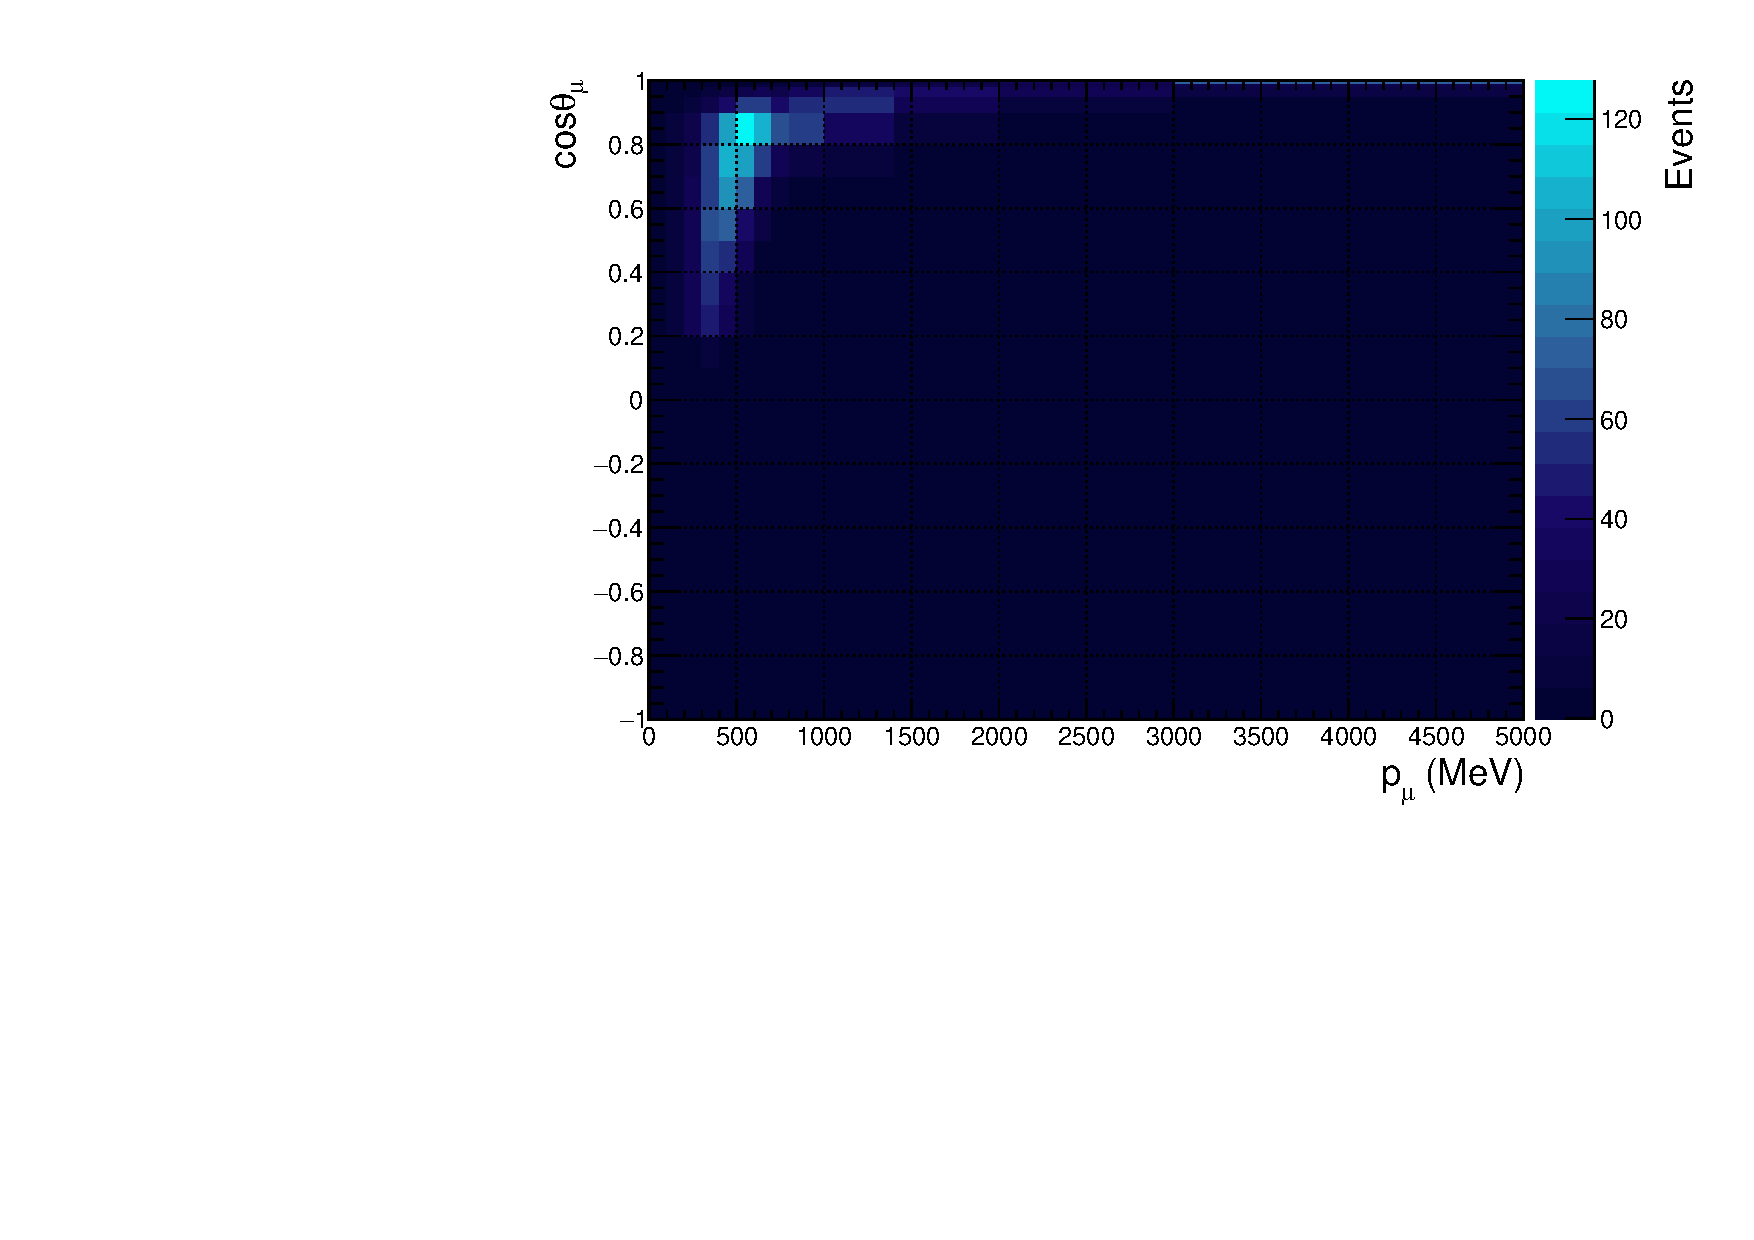
\includegraphics[width=0.9\linewidth]{figs/nd280_pmtmuu_cc0pi0p.pdf}
  \caption{CC 0$\pi$ 0p}
\end{subfigure}
\begin{subfigure}{.49\textwidth}
  \centering
  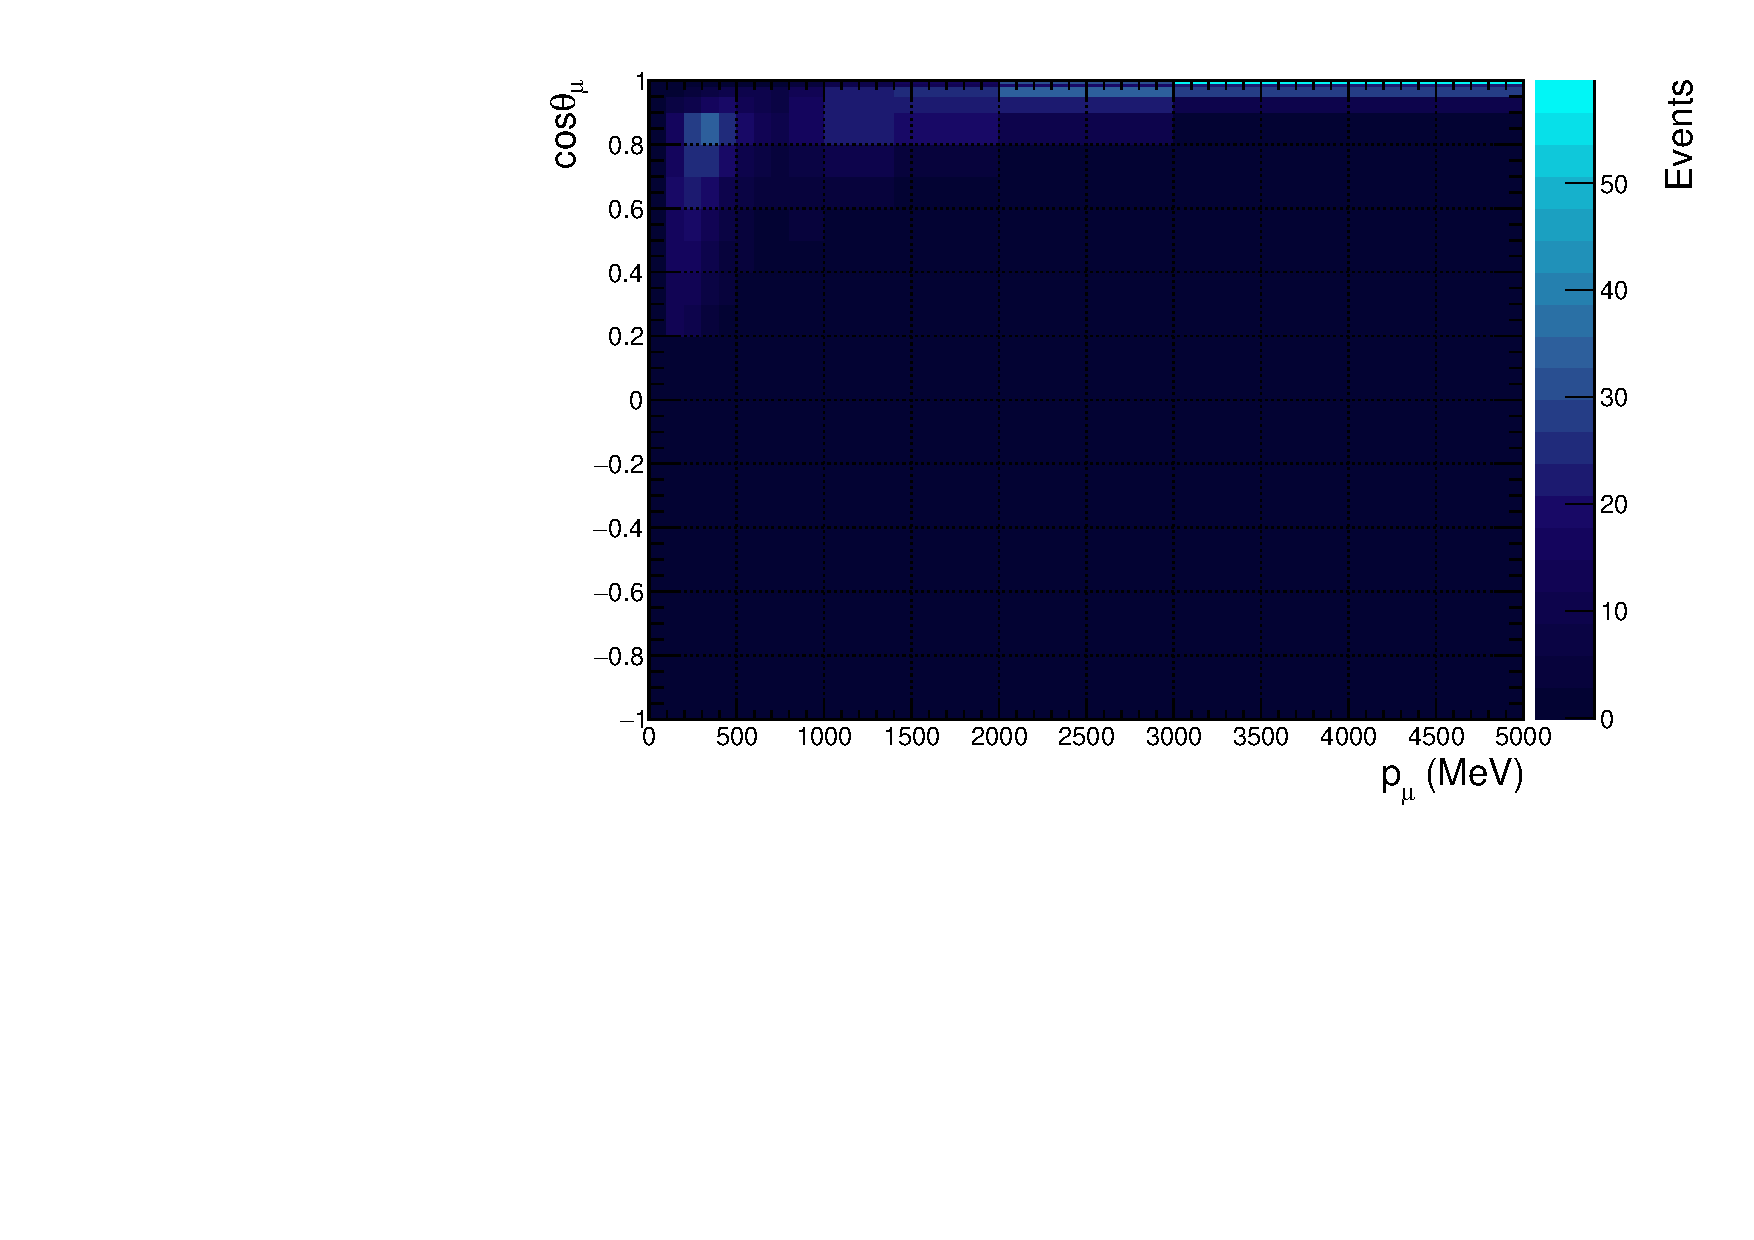
\includegraphics[width=0.9\linewidth]{figs/nd280_pmtmuu_cc1pi0p.pdf}
  \caption{CC 1$\pi$ 0p}
\end{subfigure}
\begin{subfigure}{.49\textwidth}
  \centering
  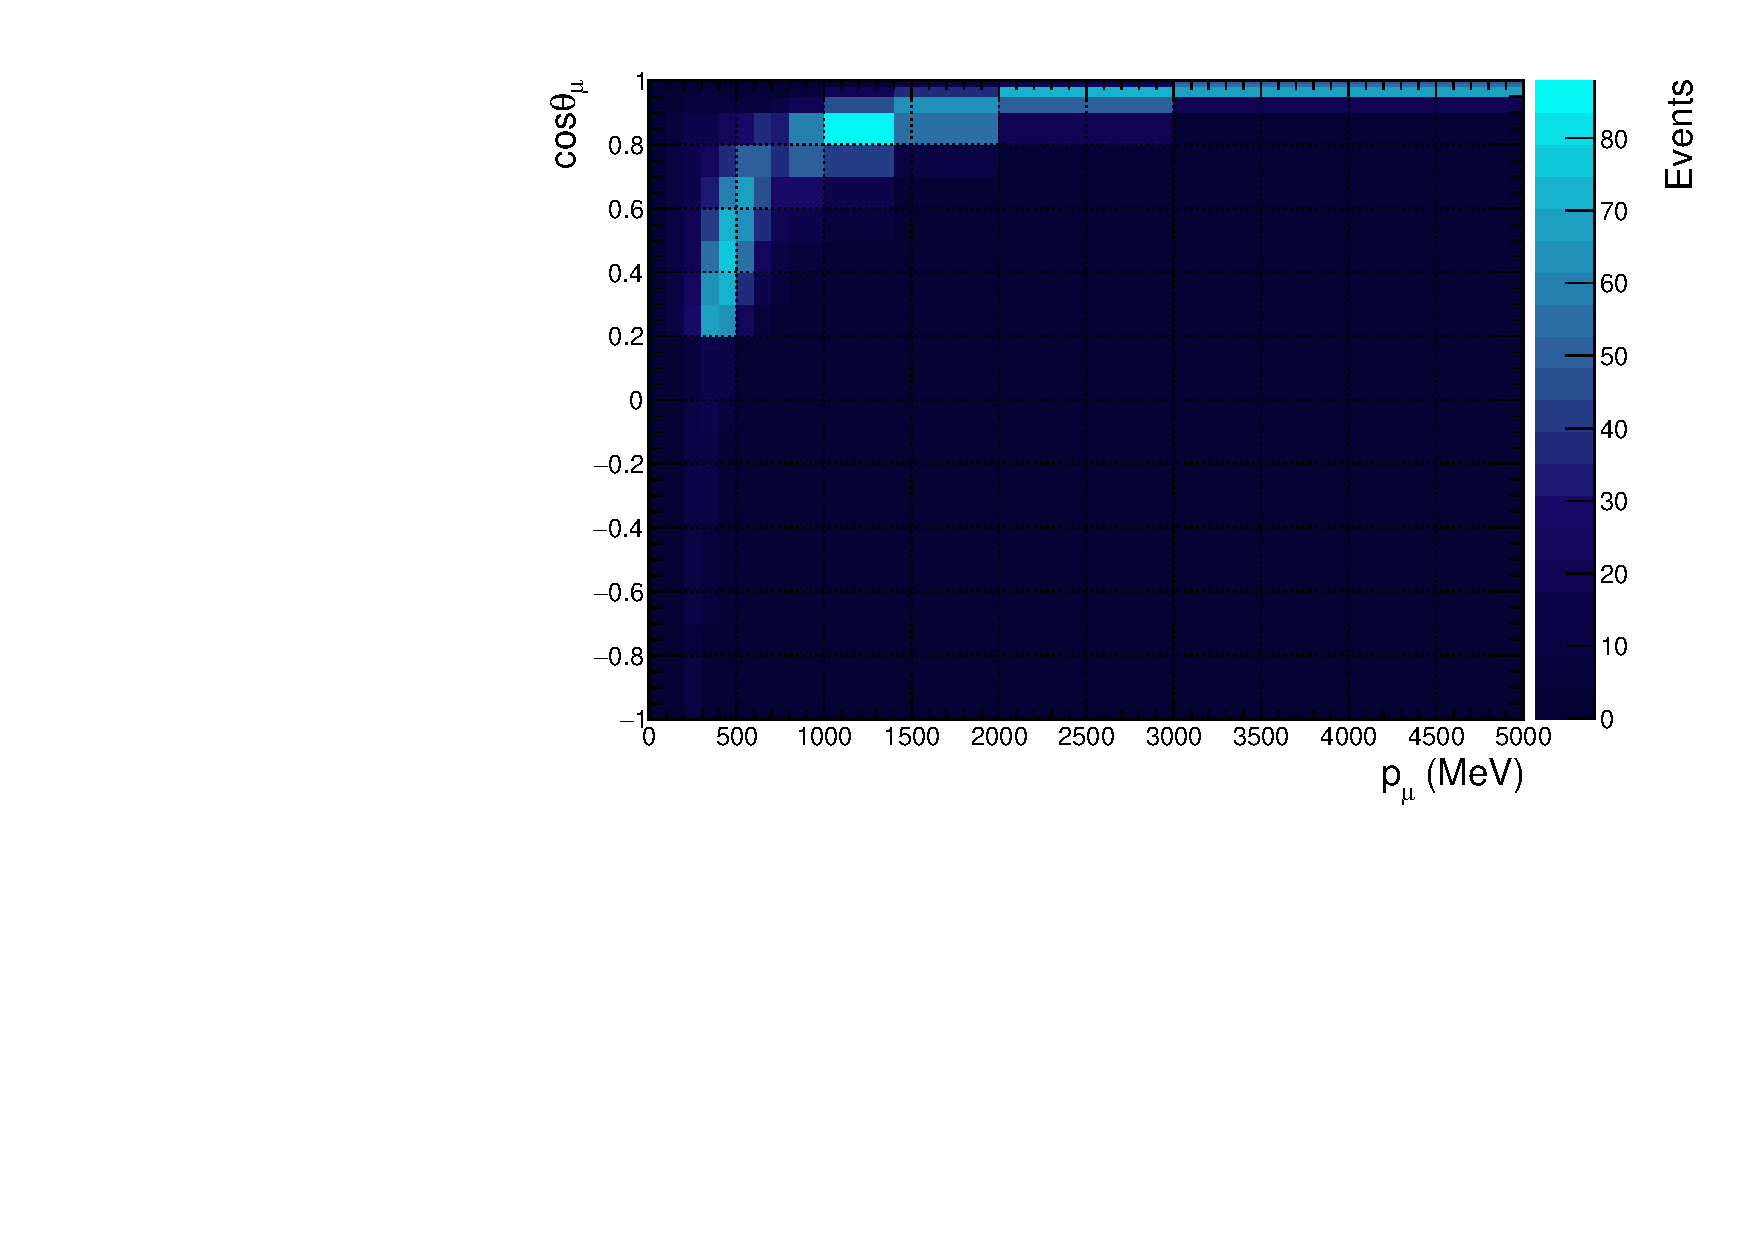
\includegraphics[width=0.9\linewidth]{figs/nd280_pmtmuu_cc0pi1p.pdf}
  \caption{CC 0$\pi$ 1p}
\end{subfigure}
\begin{subfigure}{.49\textwidth}
  \centering
  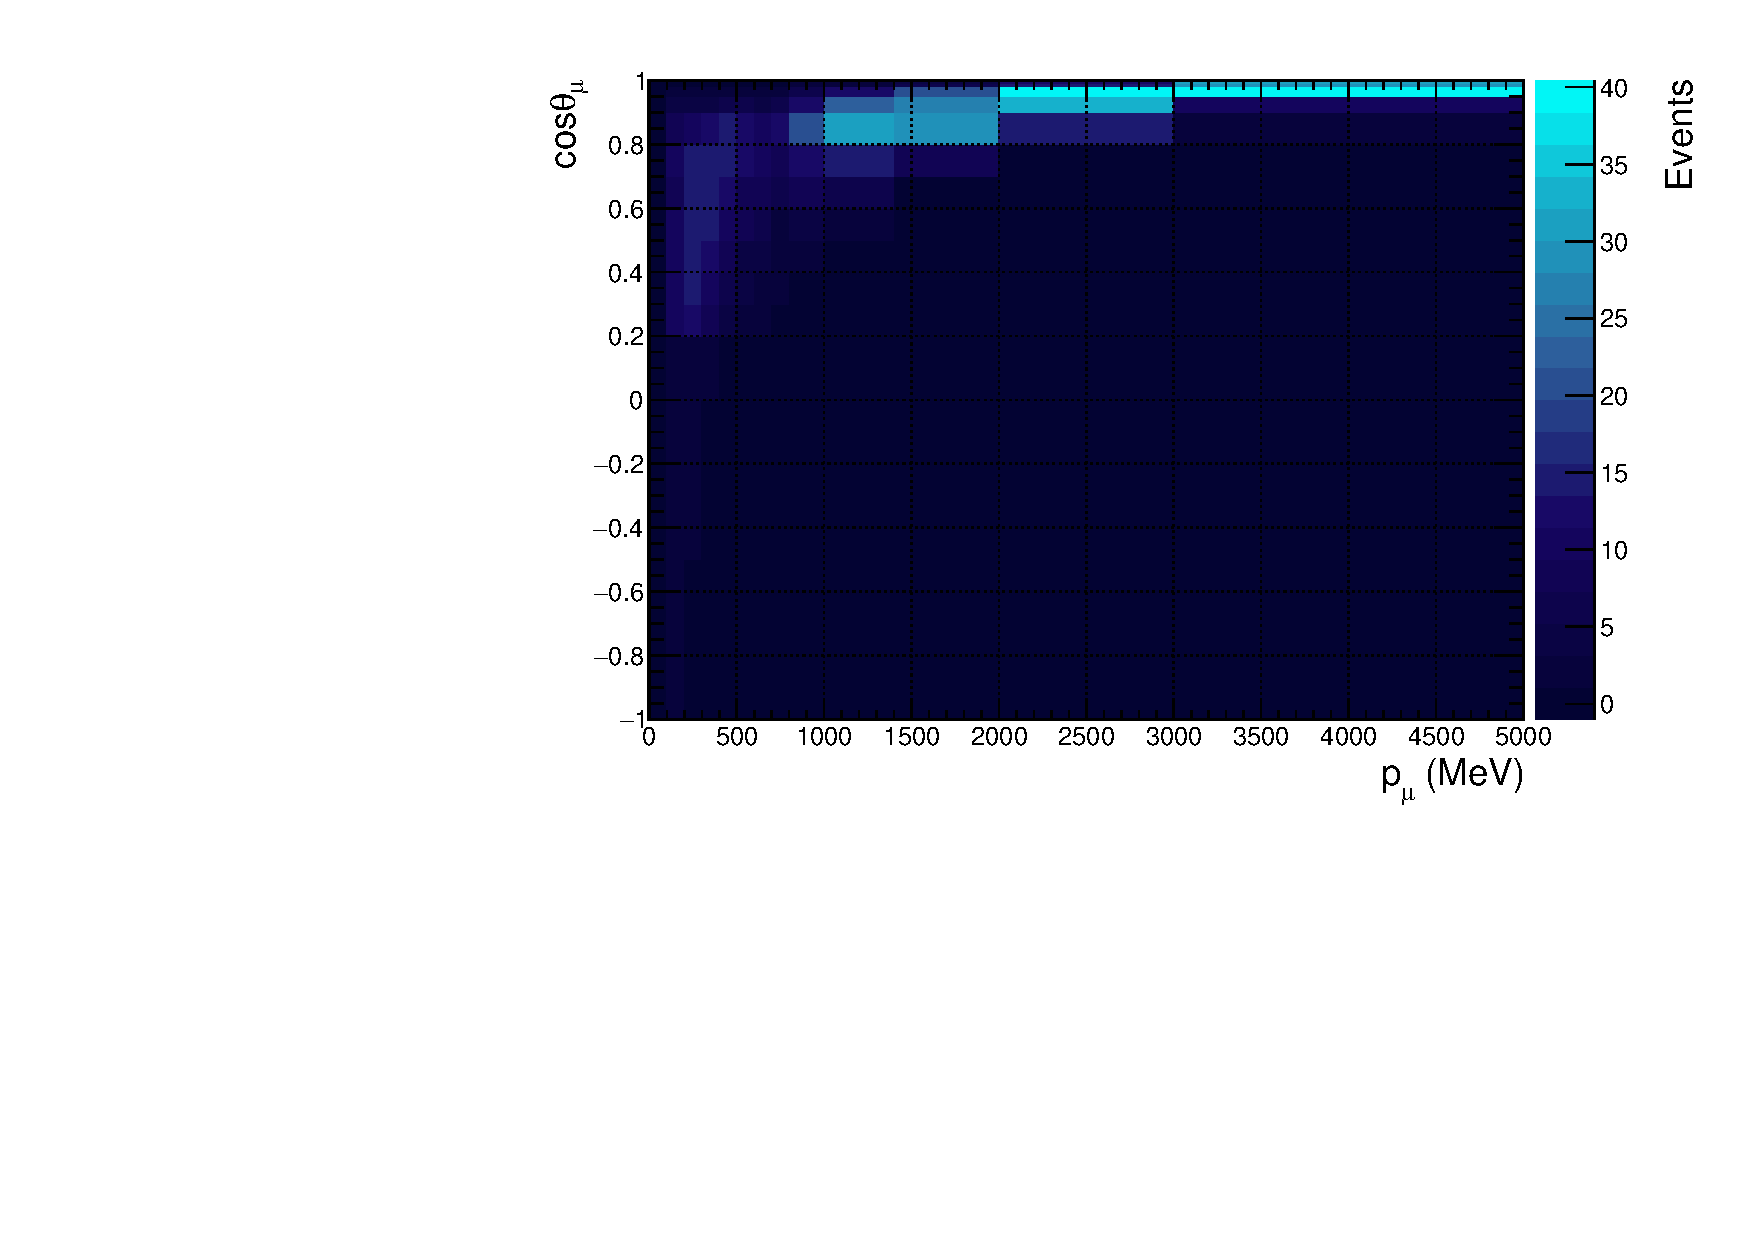
\includegraphics[width=0.9\linewidth]{figs/nd280_pmtmuu_cc1pi1p.pdf}
  \caption{CC 1$\pi$ 1p}
\end{subfigure}
\begin{subfigure}{.49\textwidth}
  \centering
  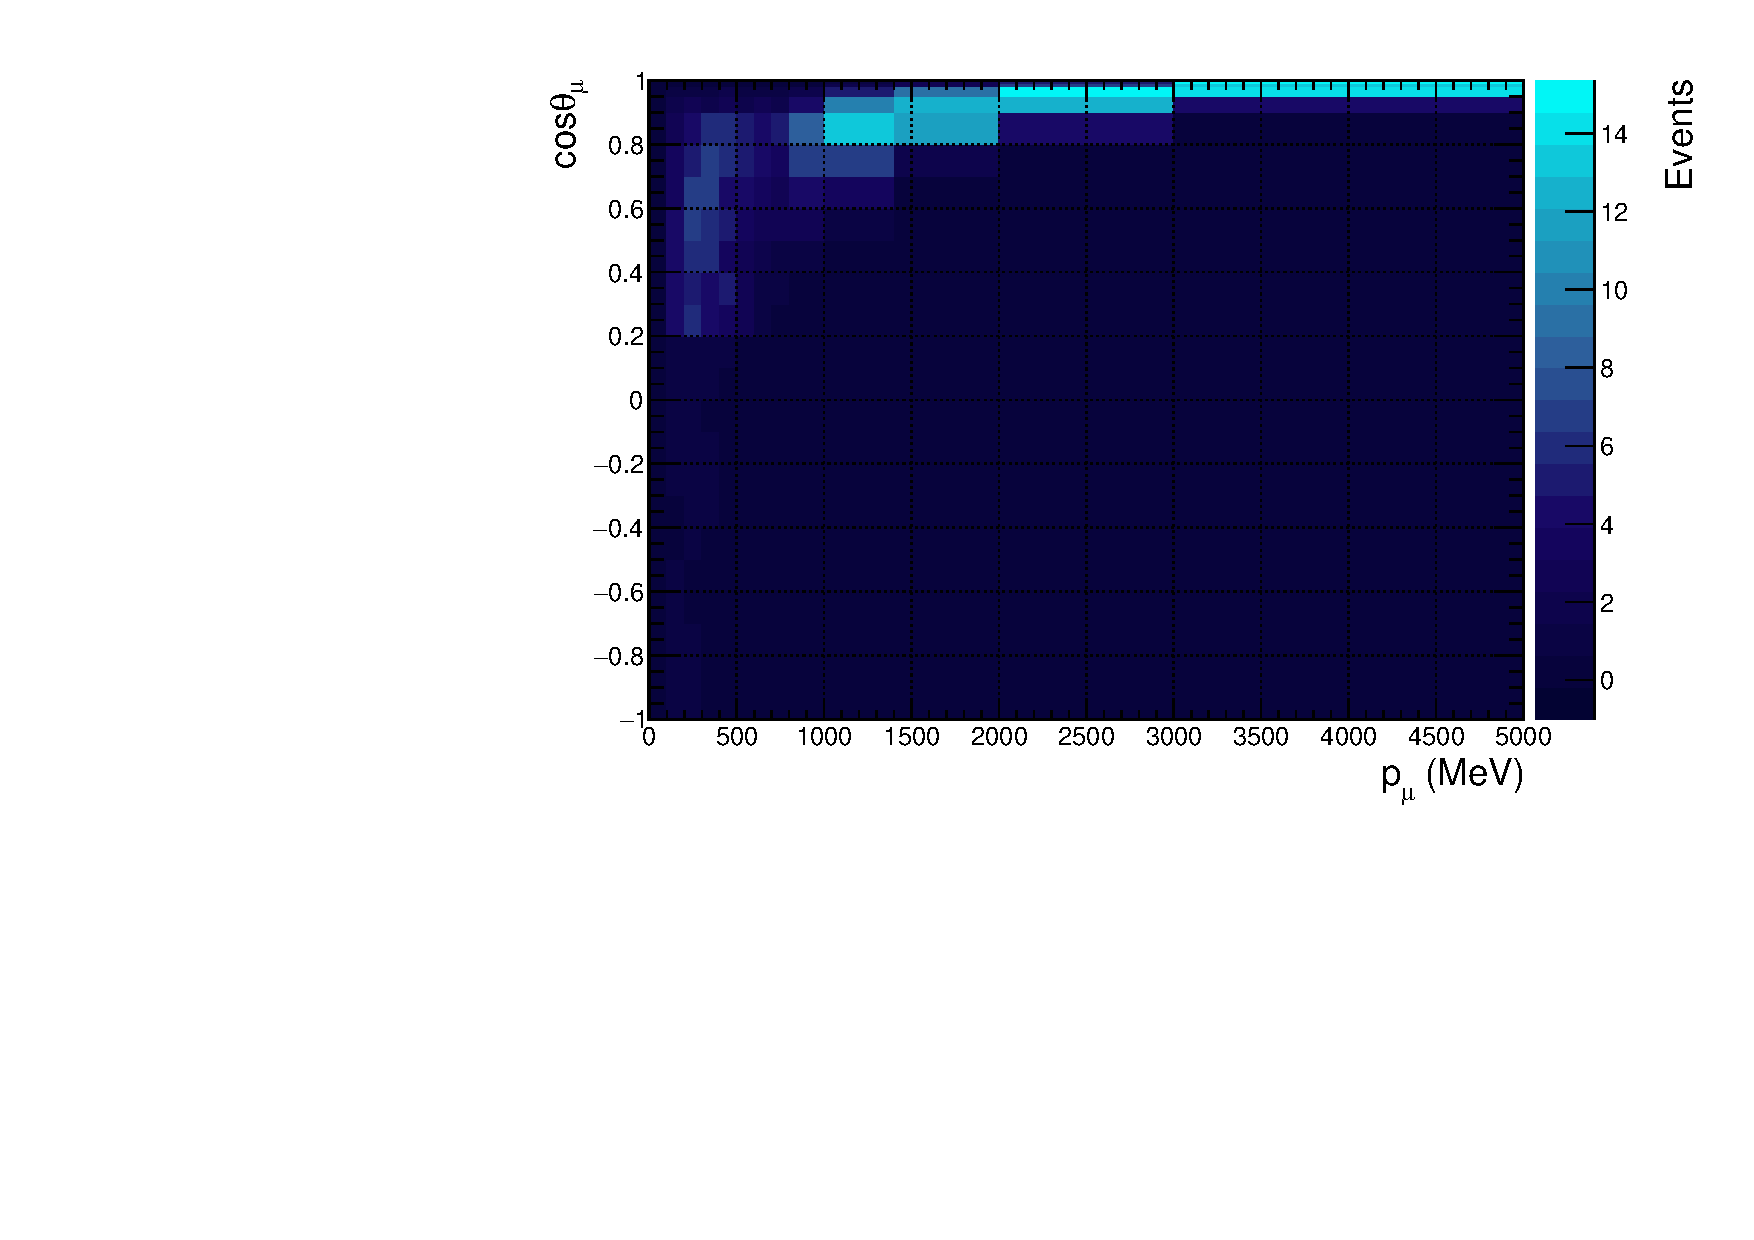
\includegraphics[width=0.9\linewidth]{figs/nd280_pmtmuu_cc0piNp.pdf}
  \caption{CC 0$\pi$ Np}
\end{subfigure}
\begin{subfigure}{.49\textwidth}
  \centering
  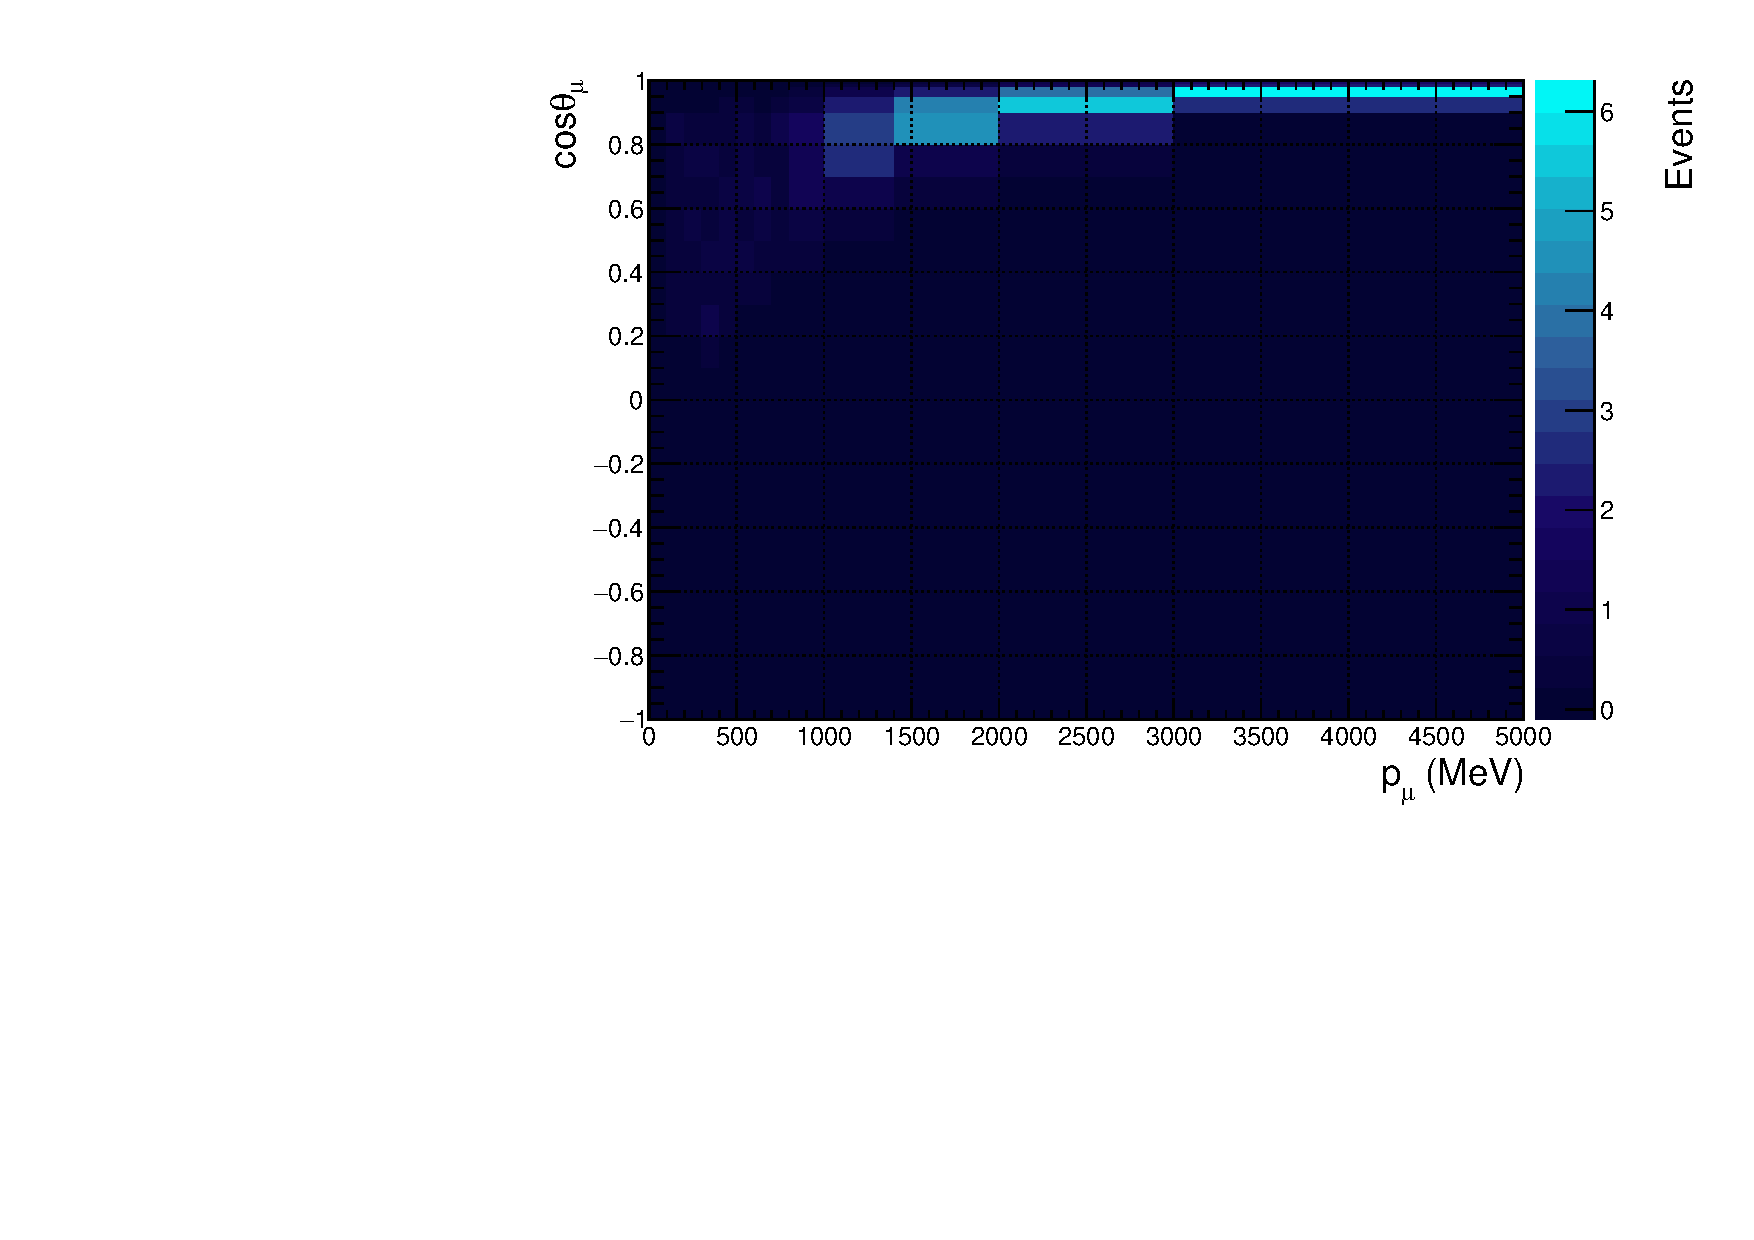
\includegraphics[width=0.9\linewidth]{figs/nd280_pmtmuu_cc1piNp.pdf}
  \caption{CC 1$\pi$ Np}
\end{subfigure}
\begin{subfigure}{.49\textwidth}
  \centering
  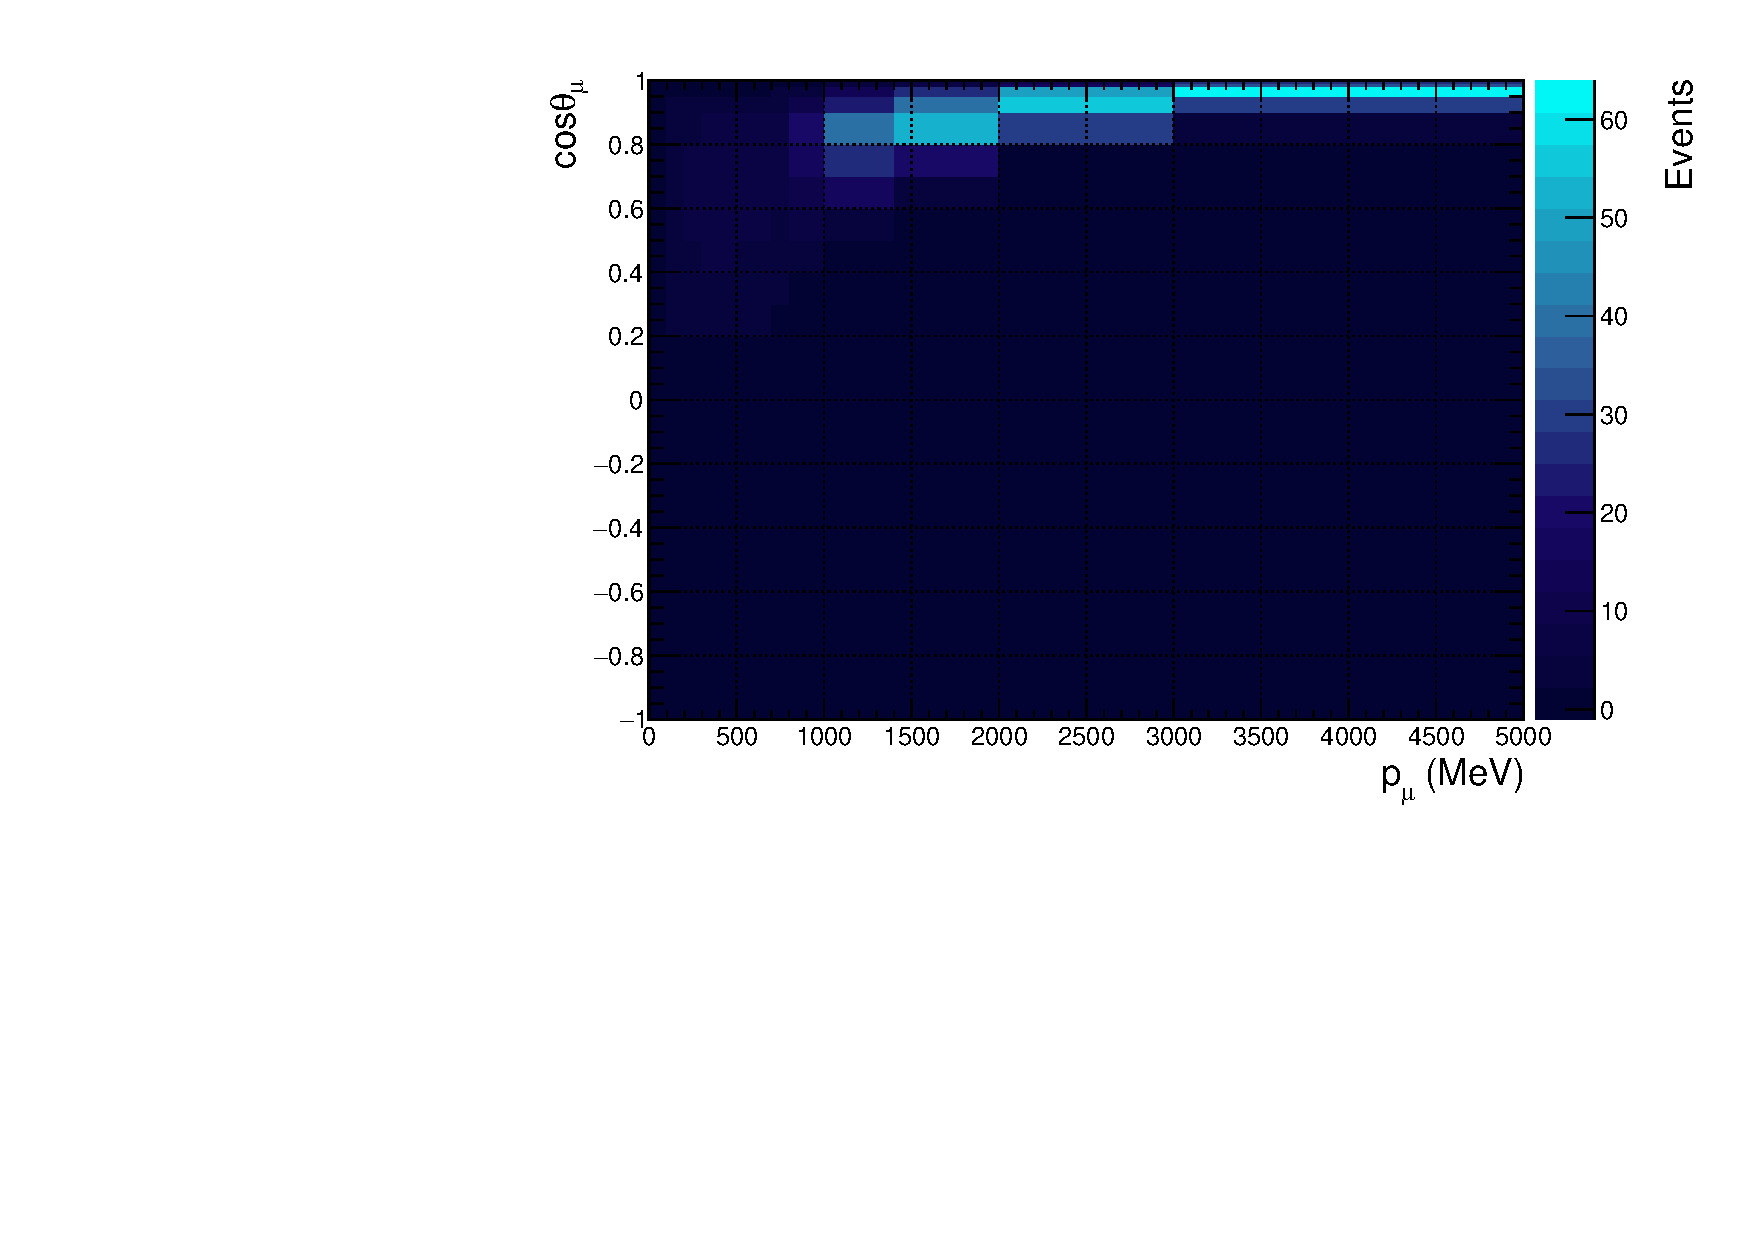
\includegraphics[width=0.9\linewidth]{figs/nd280_pmtmuu_ccOther.pdf}
  \caption{CC Other}
\end{subfigure}
\caption{True $p_{\mu}$-cos$\theta_{\mu}$ distributions for the ND280 MC.}
\label{fig:nd280PmuTmu}
\end{figure}

\begin{figure}
\centering
\begin{subfigure}{.49\textwidth}
  \centering
  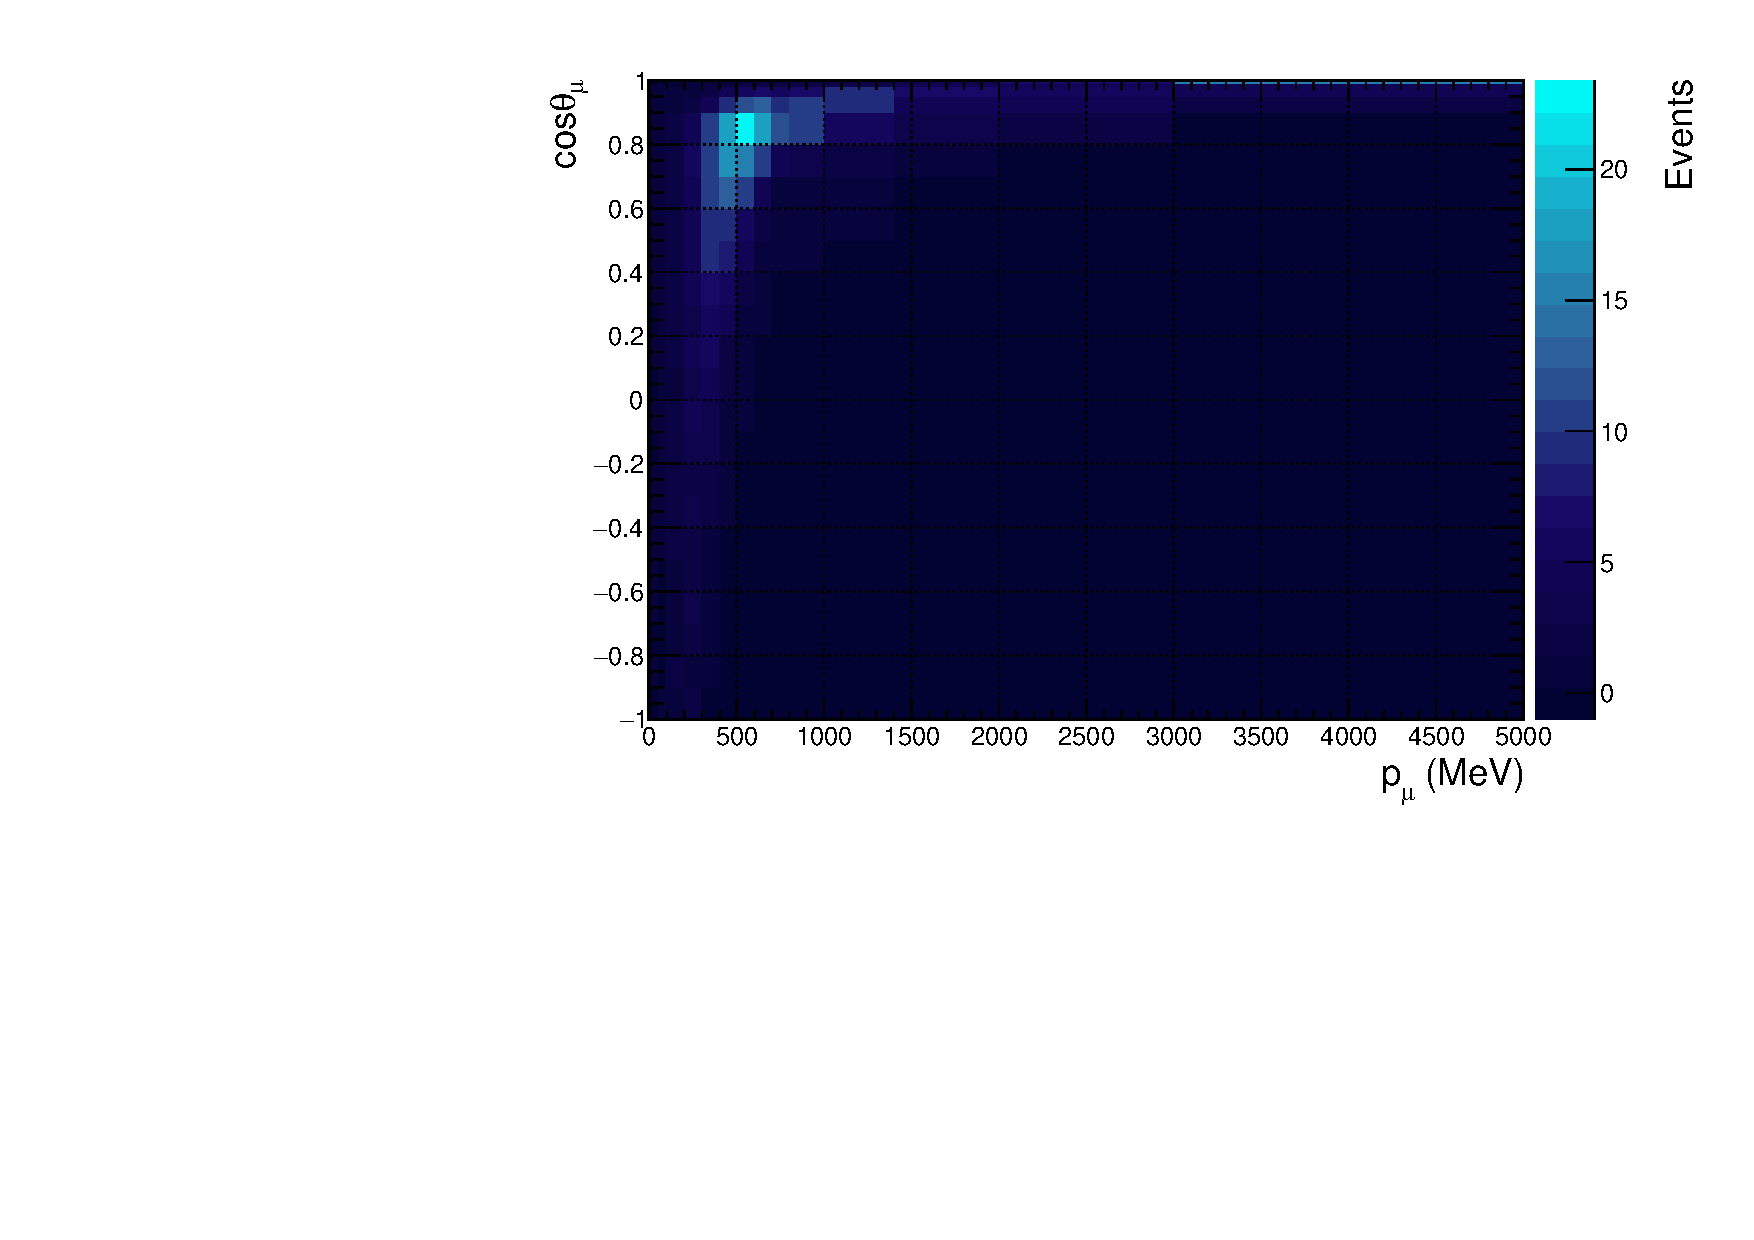
\includegraphics[width=0.9\linewidth]{figs/hptpc_pmtmuu_cc0pi0p.pdf}
  \caption{CC 0$\pi$ 0p}
\end{subfigure}
\begin{subfigure}{.49\textwidth}
  \centering
  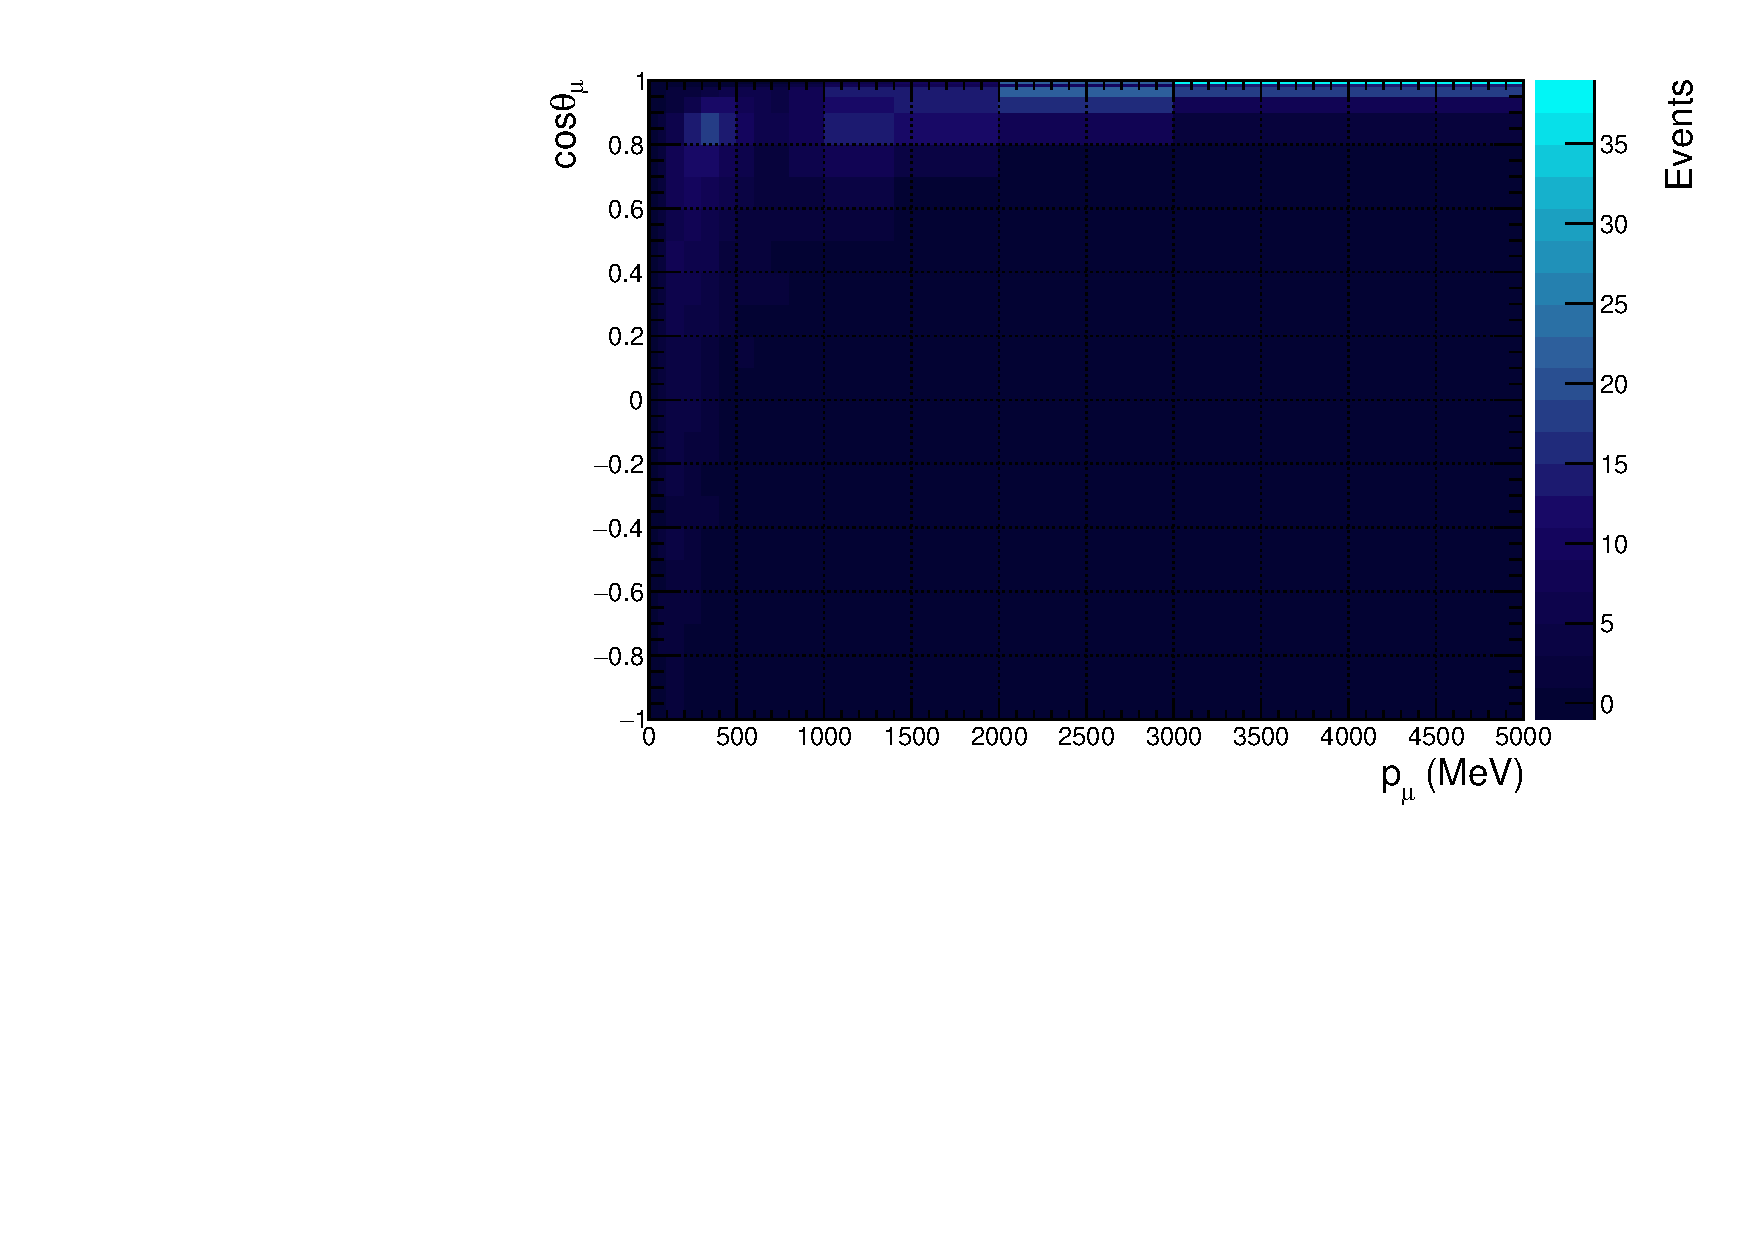
\includegraphics[width=0.9\linewidth]{figs/hptpc_pmtmuu_cc1pi0p.pdf}
  \caption{CC 1$\pi$ 0p}
\end{subfigure}
\begin{subfigure}{.49\textwidth}
  \centering
  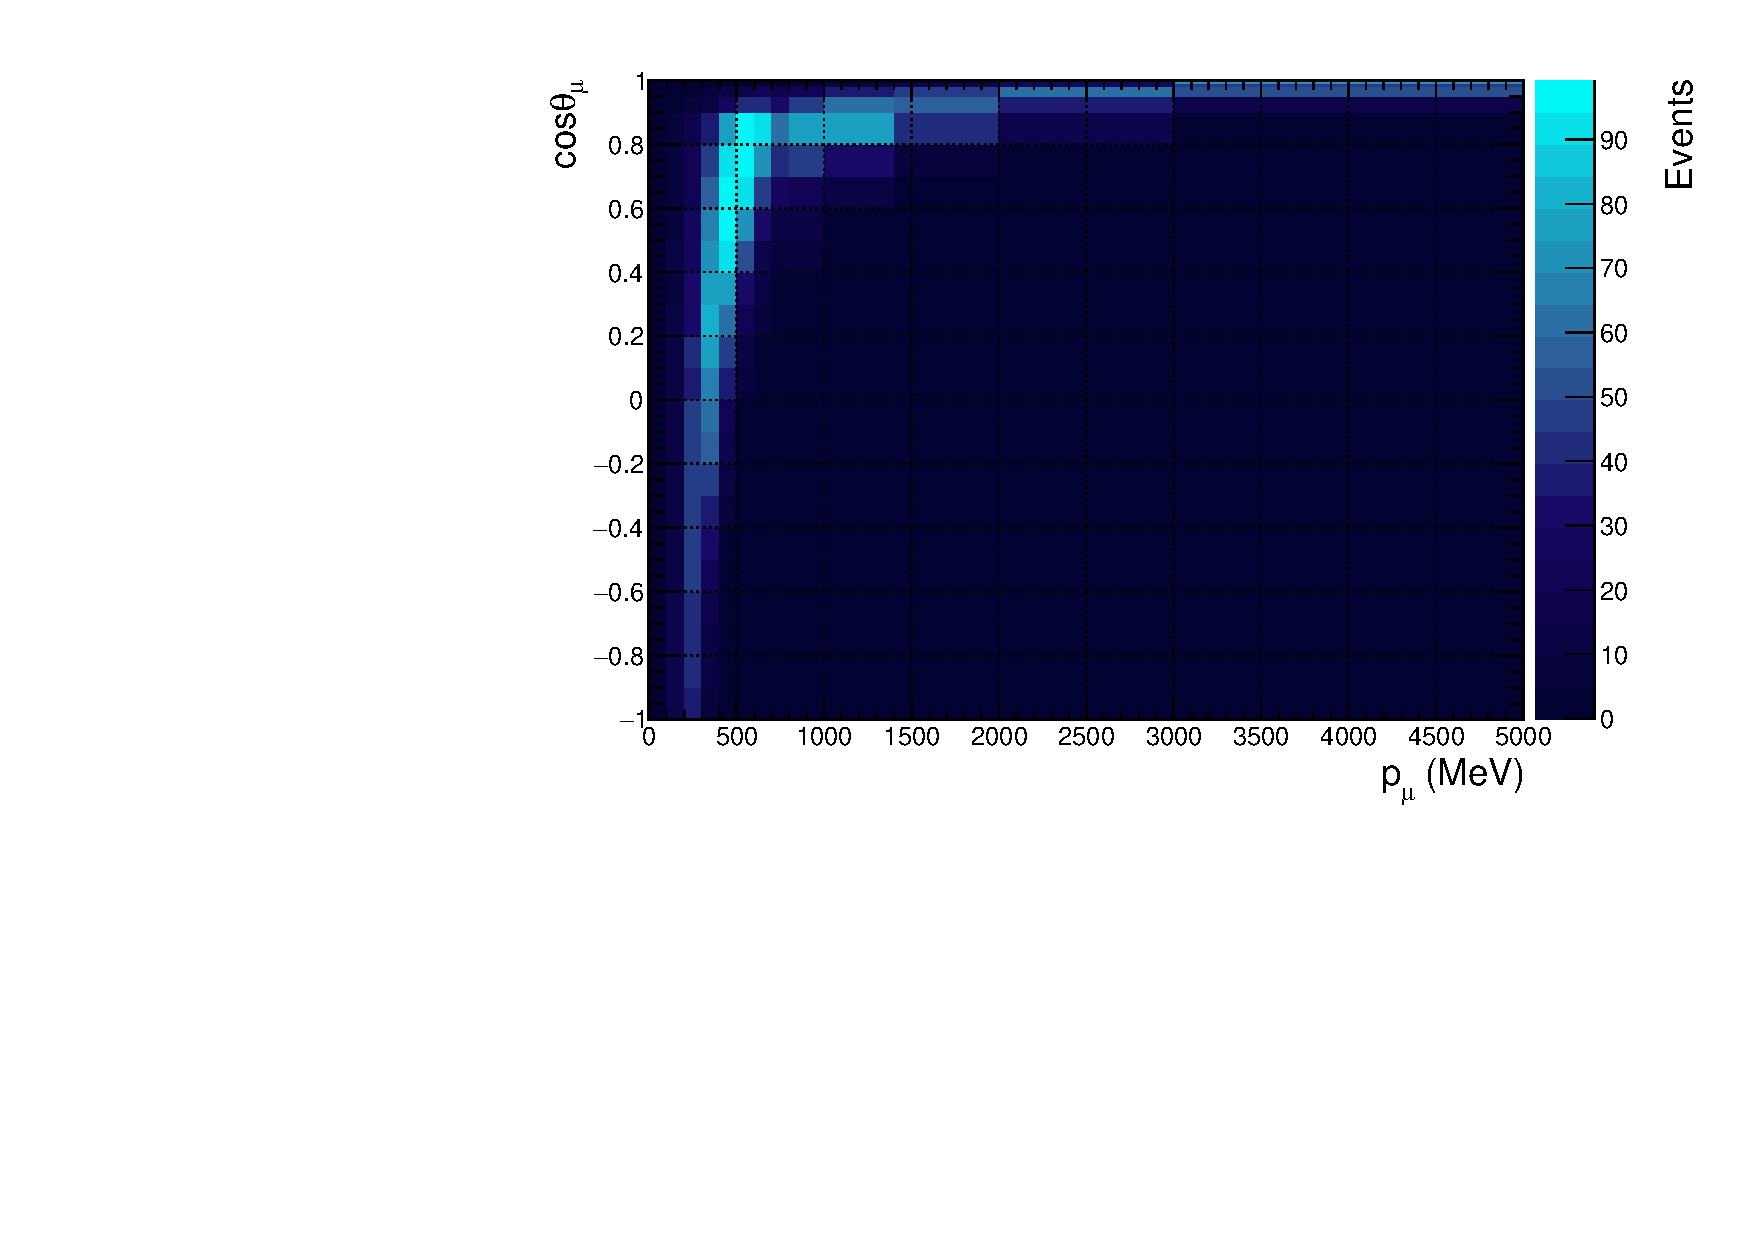
\includegraphics[width=0.9\linewidth]{figs/hptpc_pmtmuu_cc0pi1p.pdf}
  \caption{CC 0$\pi$ 1p}
\end{subfigure}
\begin{subfigure}{.49\textwidth}
  \centering
  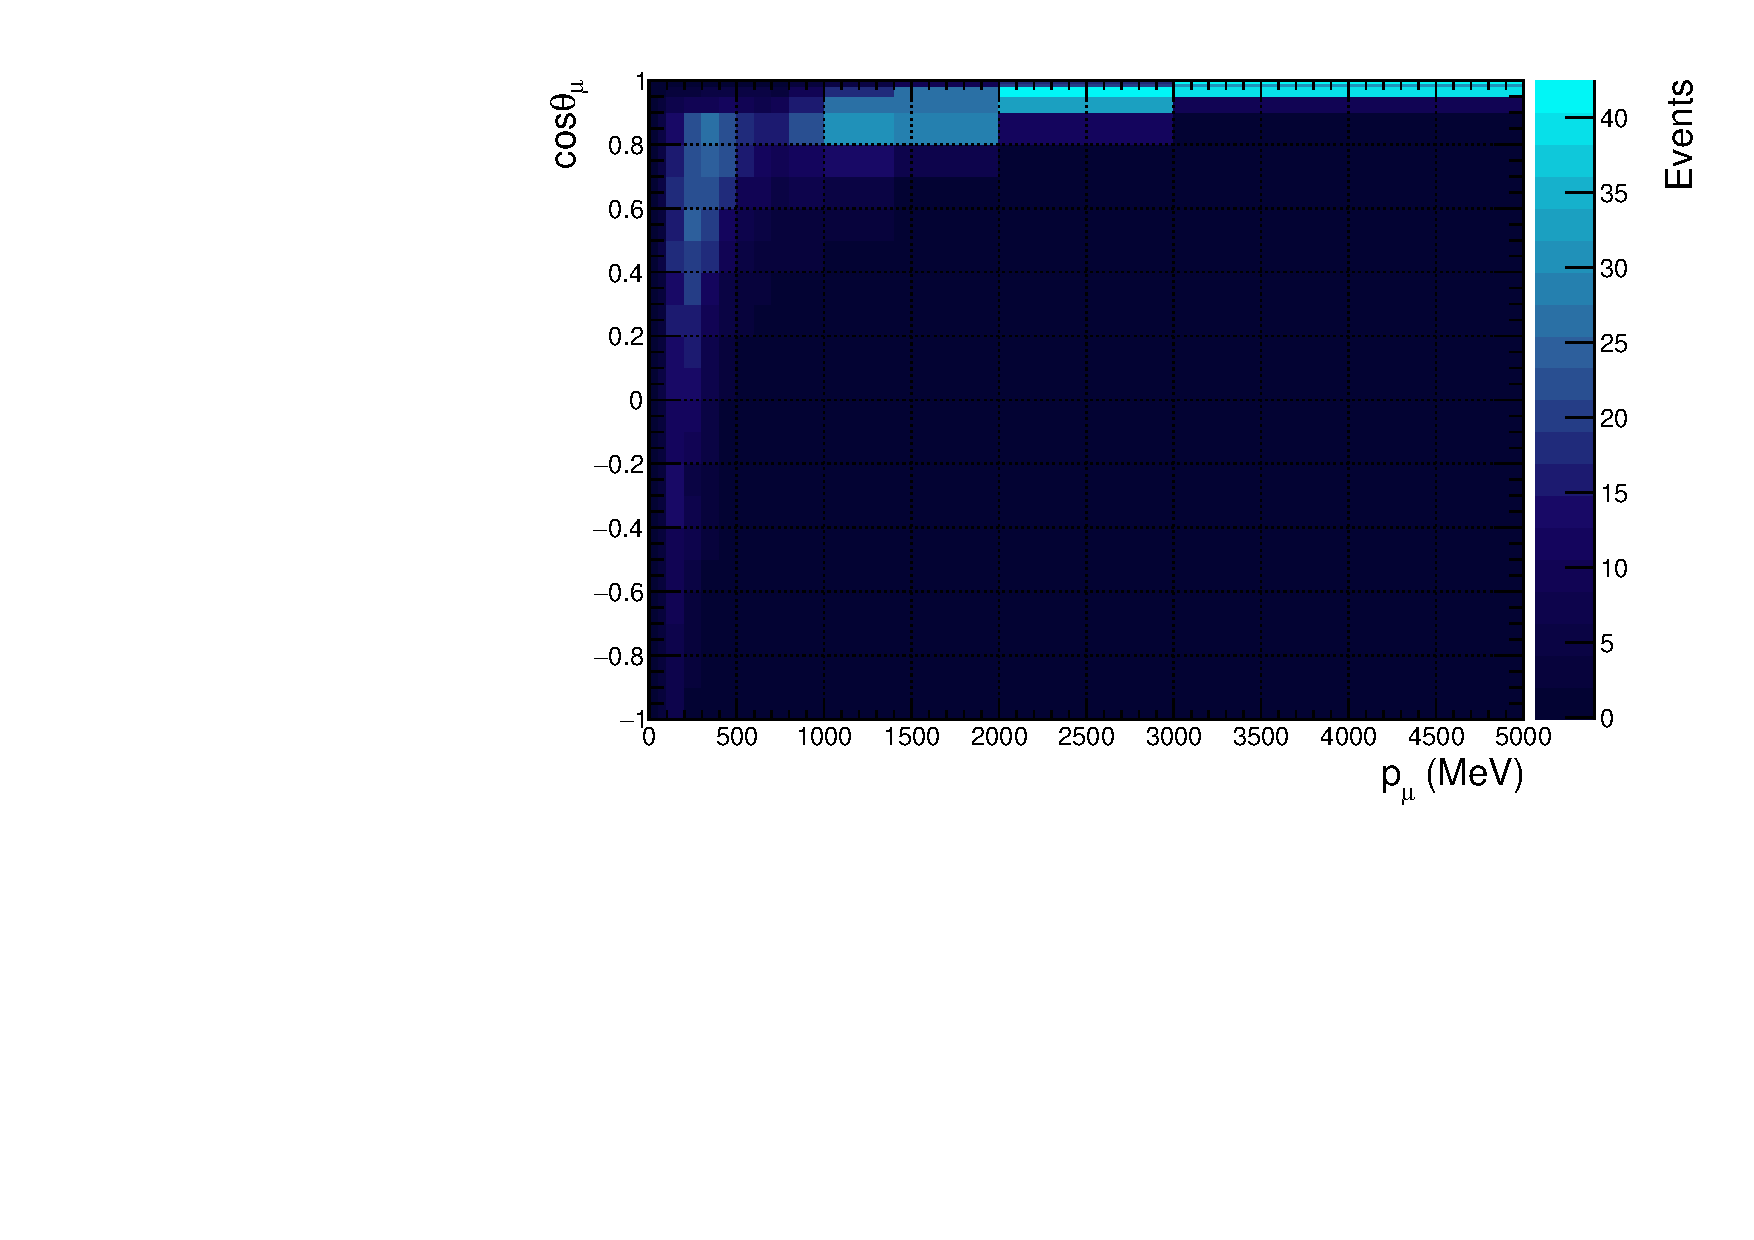
\includegraphics[width=0.9\linewidth]{figs/hptpc_pmtmuu_cc1pi1p.pdf}
  \caption{CC 1$\pi$ 1p}
\end{subfigure}
\begin{subfigure}{.49\textwidth}
  \centering
  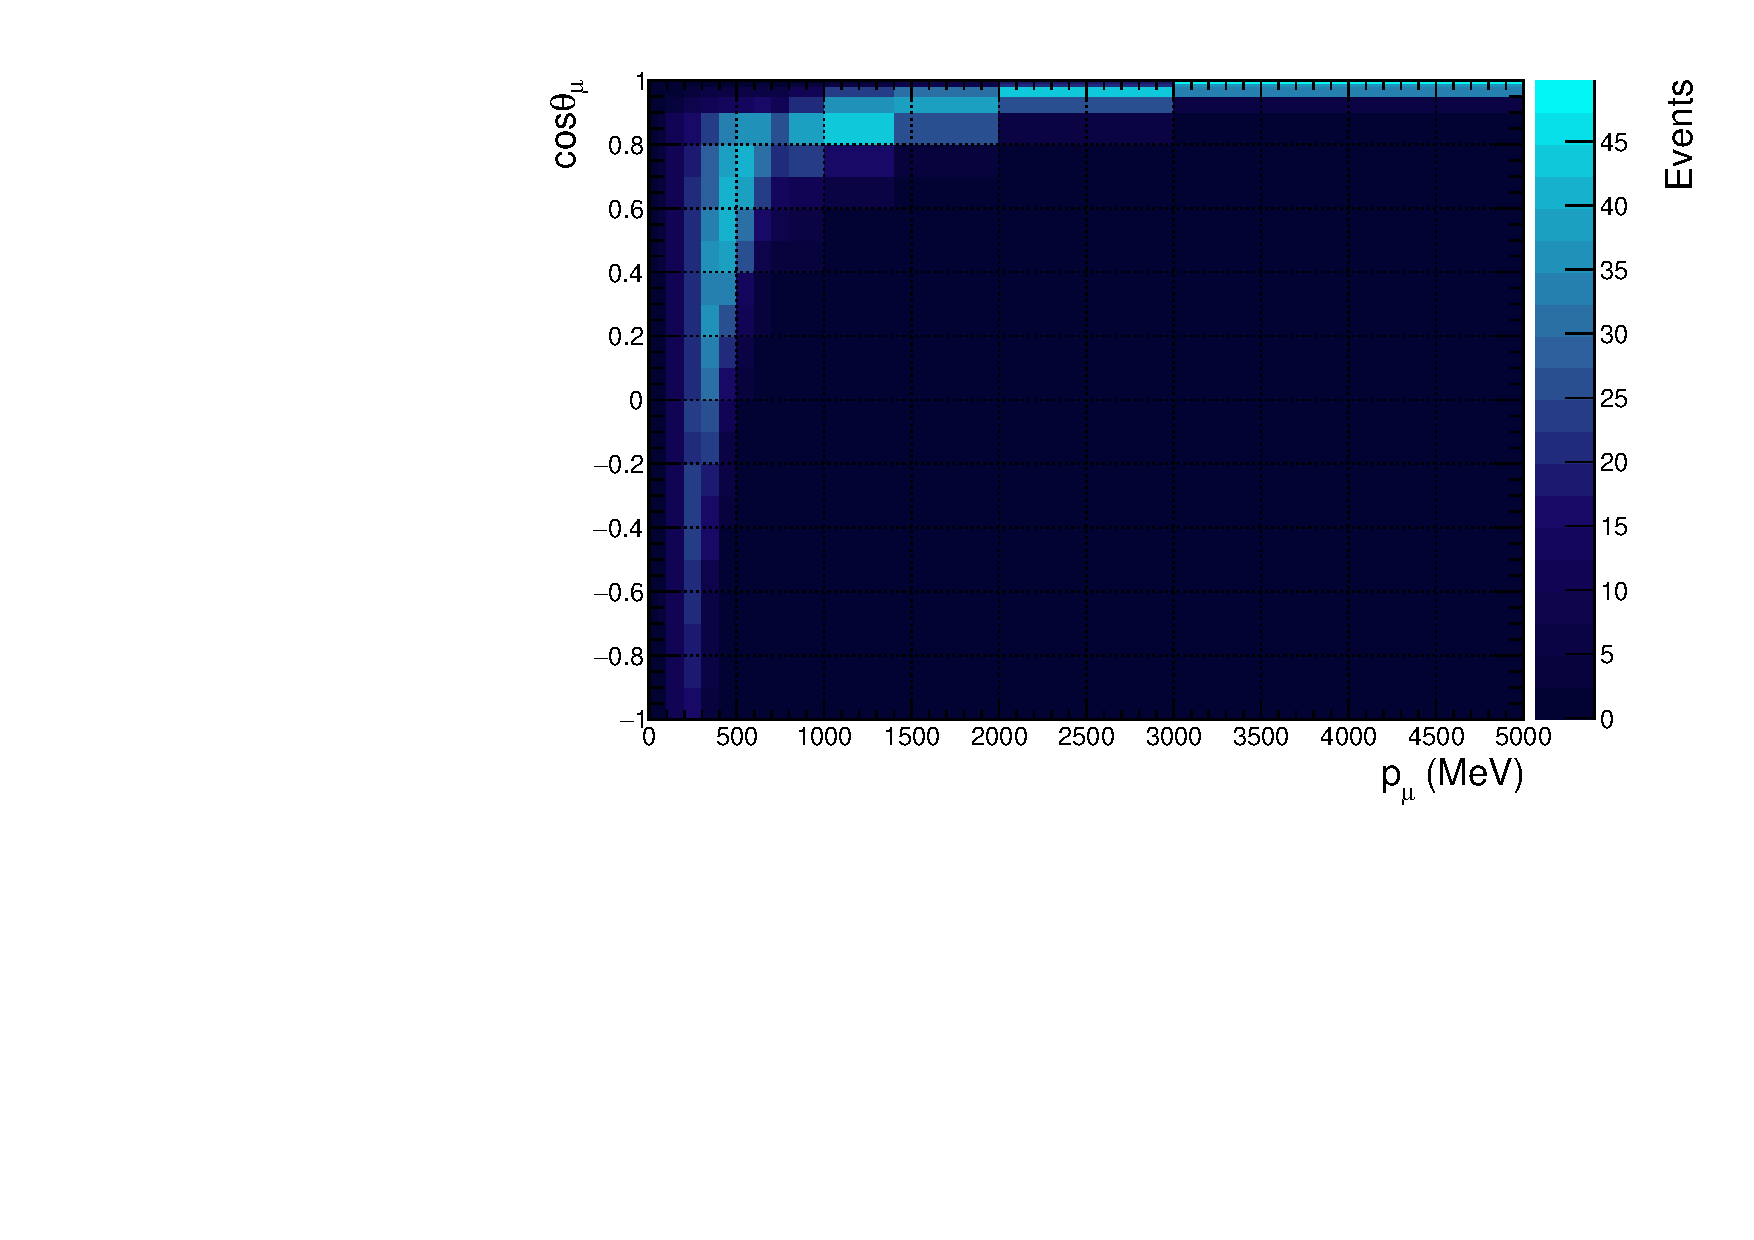
\includegraphics[width=0.9\linewidth]{figs/hptpc_pmtmuu_cc0piNp.pdf}
  \caption{CC 0$\pi$ Np}
\end{subfigure}
\begin{subfigure}{.49\textwidth}
  \centering
  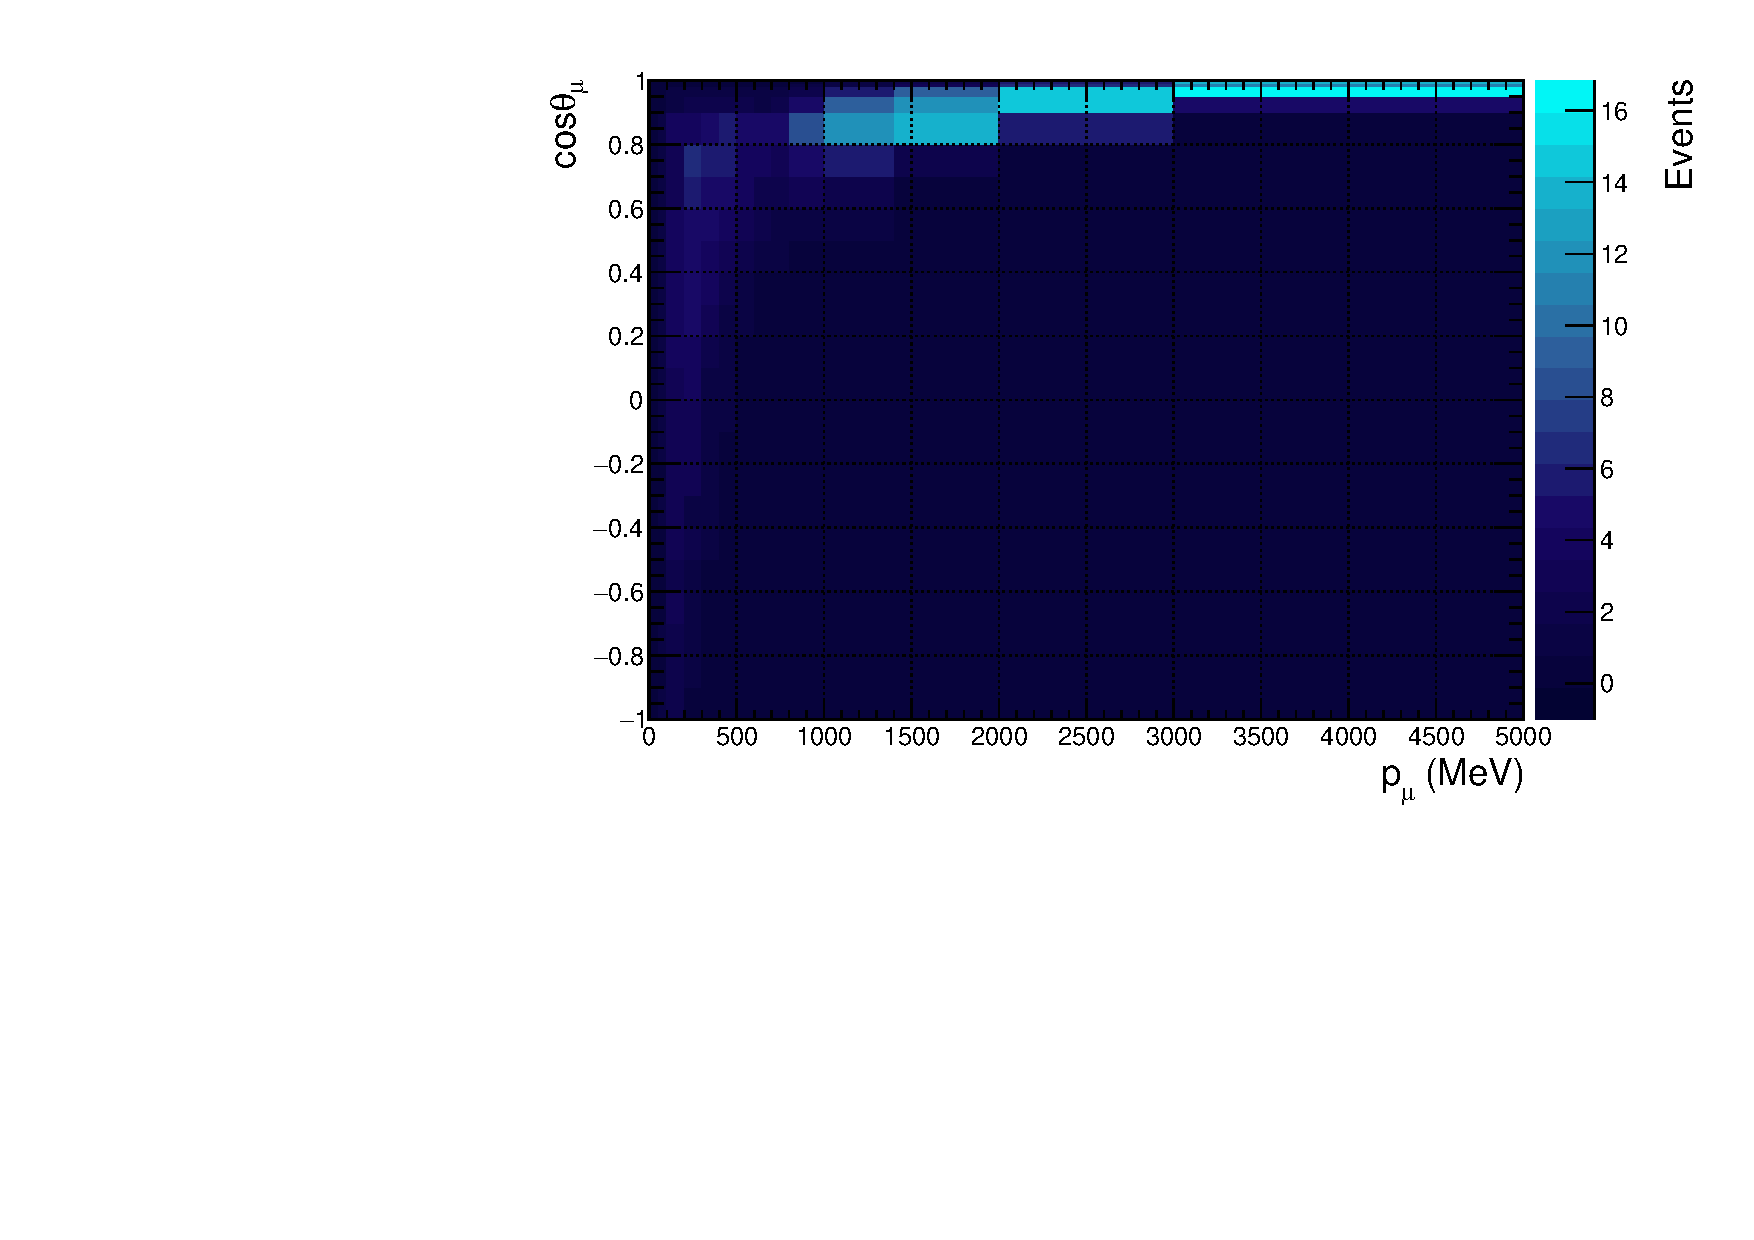
\includegraphics[width=0.9\linewidth]{figs/hptpc_pmtmuu_cc1piNp.pdf}
  \caption{CC 1$\pi$ Np}
\end{subfigure}
\begin{subfigure}{.49\textwidth}
  \centering
  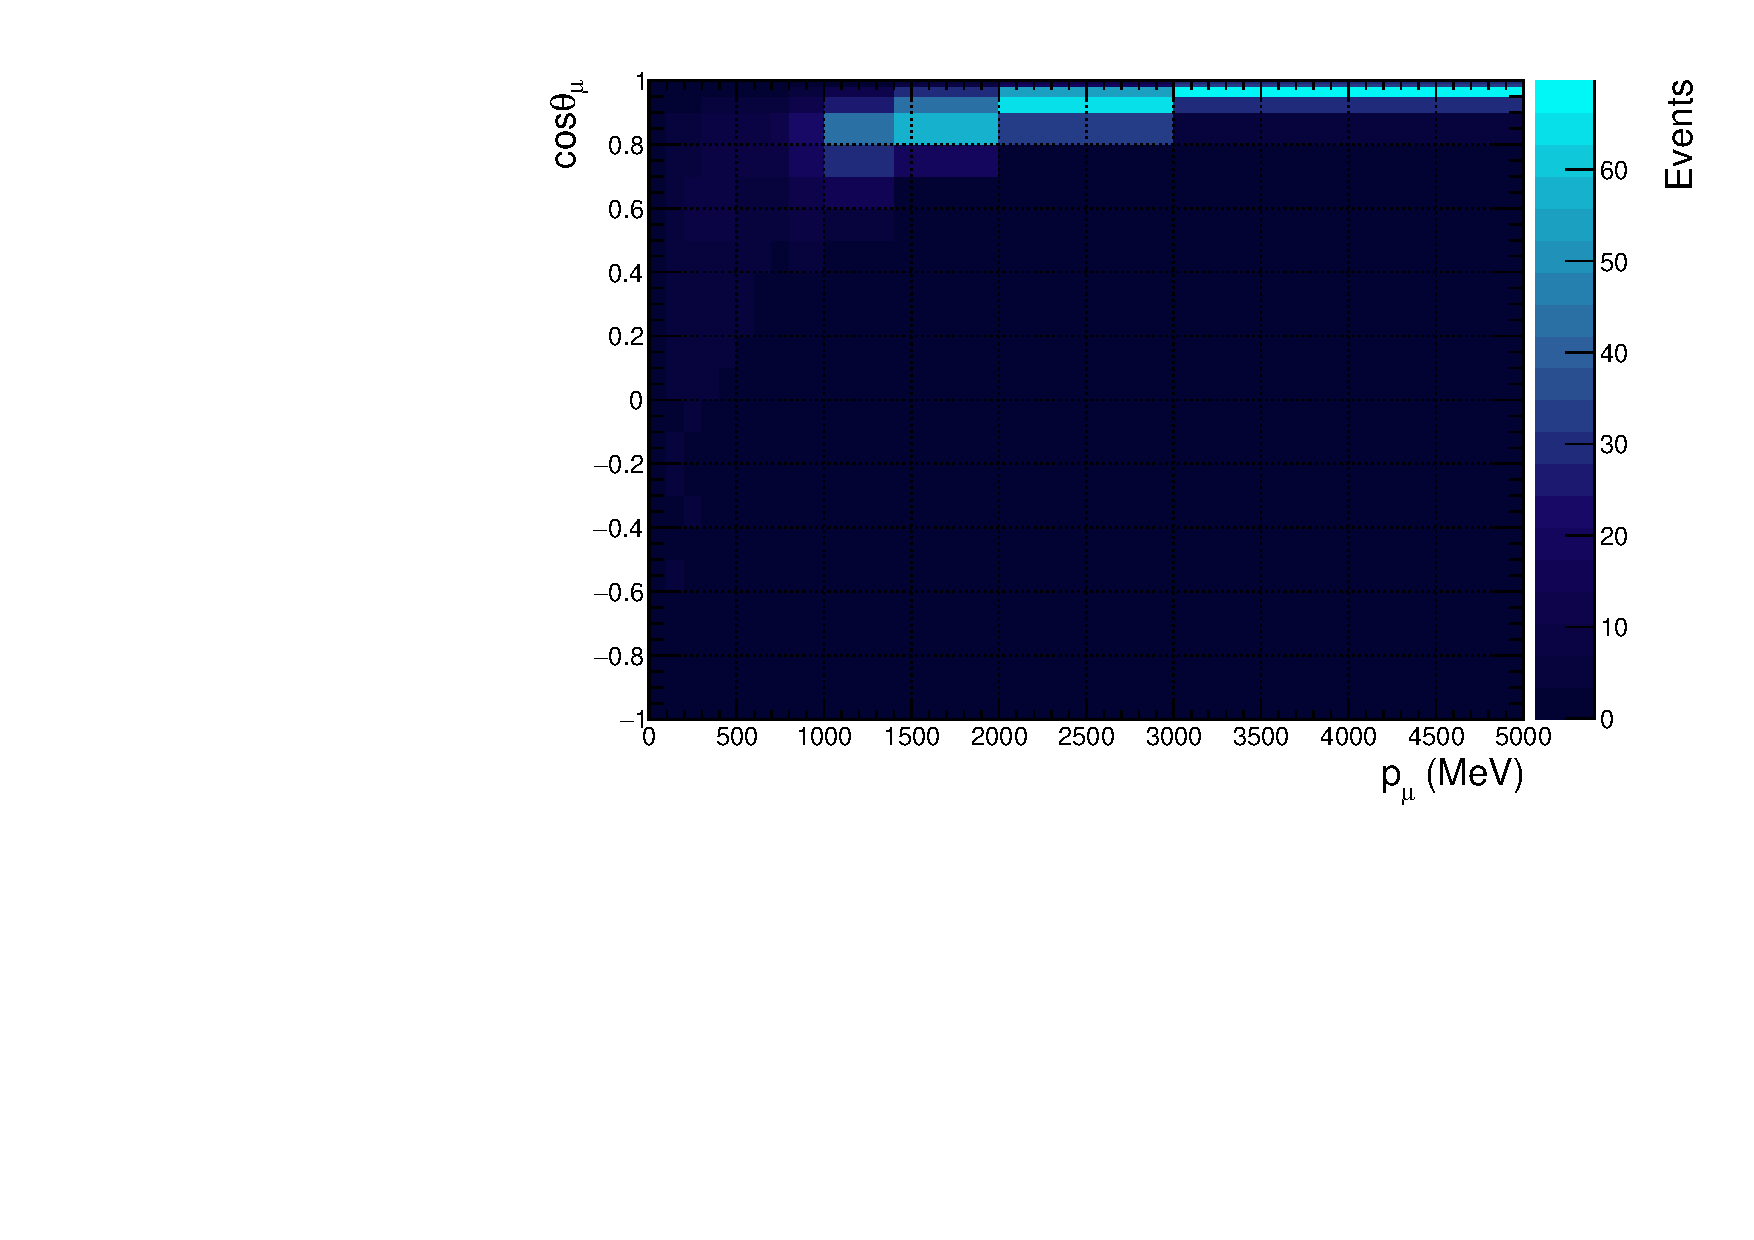
\includegraphics[width=0.9\linewidth]{figs/hptpc_pmtmuu_ccOther.pdf}
  \caption{CC Other}
\end{subfigure}
\caption{True $p_{\mu}$-cos$\theta_{\mu}$ distributions for the HPTPC MC.}
\label{fig:hptpcPmuTmu}
\end{figure}

The distributions of CC 0$\pi$ 0p and CC 0$\pi$ 1p samples are similar for the two detectors, but the normalisations are higher for ND280. The 1p and Np samples have significantly more backward going low momentum events in the HPTPC distirbutions than ND280. This is because if a proton is detected in an event with a low momentum lepton, the proton momentum is also likely to be low, and so more will be below the ND280 detection threshold. The shape of the CC Other distributions are similar, but there is a slightly higher normalisation for HPTPC.

The full potential sensitivity of the HPTPC to resolving nuclear model tensions cannot be achieved with lepton kinematics alone. To investigate the impact of using hadronic information in interactions, $\pm1\sigma$ parameter variations were run on the HPTPC MC in different combinations of single transverse variables, and lepton, proton, and pion momentum and angle. The process was the same as that described in Section \ref{sec:sigvar}, but events were binned in different variables.

The transverse variables are calculated for each event from the smeared true lepton momentum and angle. 

For each sample, the combination of interaction parameter and kinematic variables which caused the largest changed in the total number of events is shown in Table \ref{tab:hptpcsigvar}. 

\begin{center}
\begin{table}
\center
\begin{tabular}{l ||c c}
\hline \hline
\textbf{Sample} & \textbf{Parameter} & \textbf{Kinematic Variables} \\
 \hline \hline
CC 0$\pi$ 0p & $M_{A}^{RES}$ & $p_{\mu}$-cos$\theta_{\mu}$\\
CC 0$\pi$ 1p & 2p2h Shape C & $p_{p}$-cos$\theta_{\mu}$\\
CC 0$\pi$ Np & $M_{A}^{QE}$ & $p_{p}$-cos$\theta_{\mu}$\\
CC 1$\pi$ 0p & $M_{A}^{RES}$ & $p_{\pi}$-cos$\theta_{\mu}$\\
CC 1$\pi$ 1p & $C_{A}^{5}$ & $\delta p_{T}$-cos$\theta_{\mu}$\\
CC 1$\pi$ Np & $C_{A}^{5}$ & $p_{p}$-cos$\theta_{\mu}$\\
CC Other & CC DIS & $p_{\mu}$-cos$\theta_{\mu}$\\
\hline \hline
\end{tabular}
\caption{Combination of kinematic variable pair and interaction parameter which caused the biggest change in the total event rate for each sample in the $\pm1\sigma$ parameter variations.}
\label{tab:hptpcsigvar}
\end{table}
\end{center}

Interestingly, for each sample one of the pair of kinematic that  variables that cause the biggest change in the event rates in the parameter variations is either the lepton momentum or angle. This is likely because these variables can be measured with the best resolution by the detectors.

The distributions in these pairs of kinematics for the HPTPC MC samples are shown in Figure \ref{fig:hptpcsigvar}.

\begin{figure}
\centering
\begin{subfigure}{.49\textwidth}
  \centering
  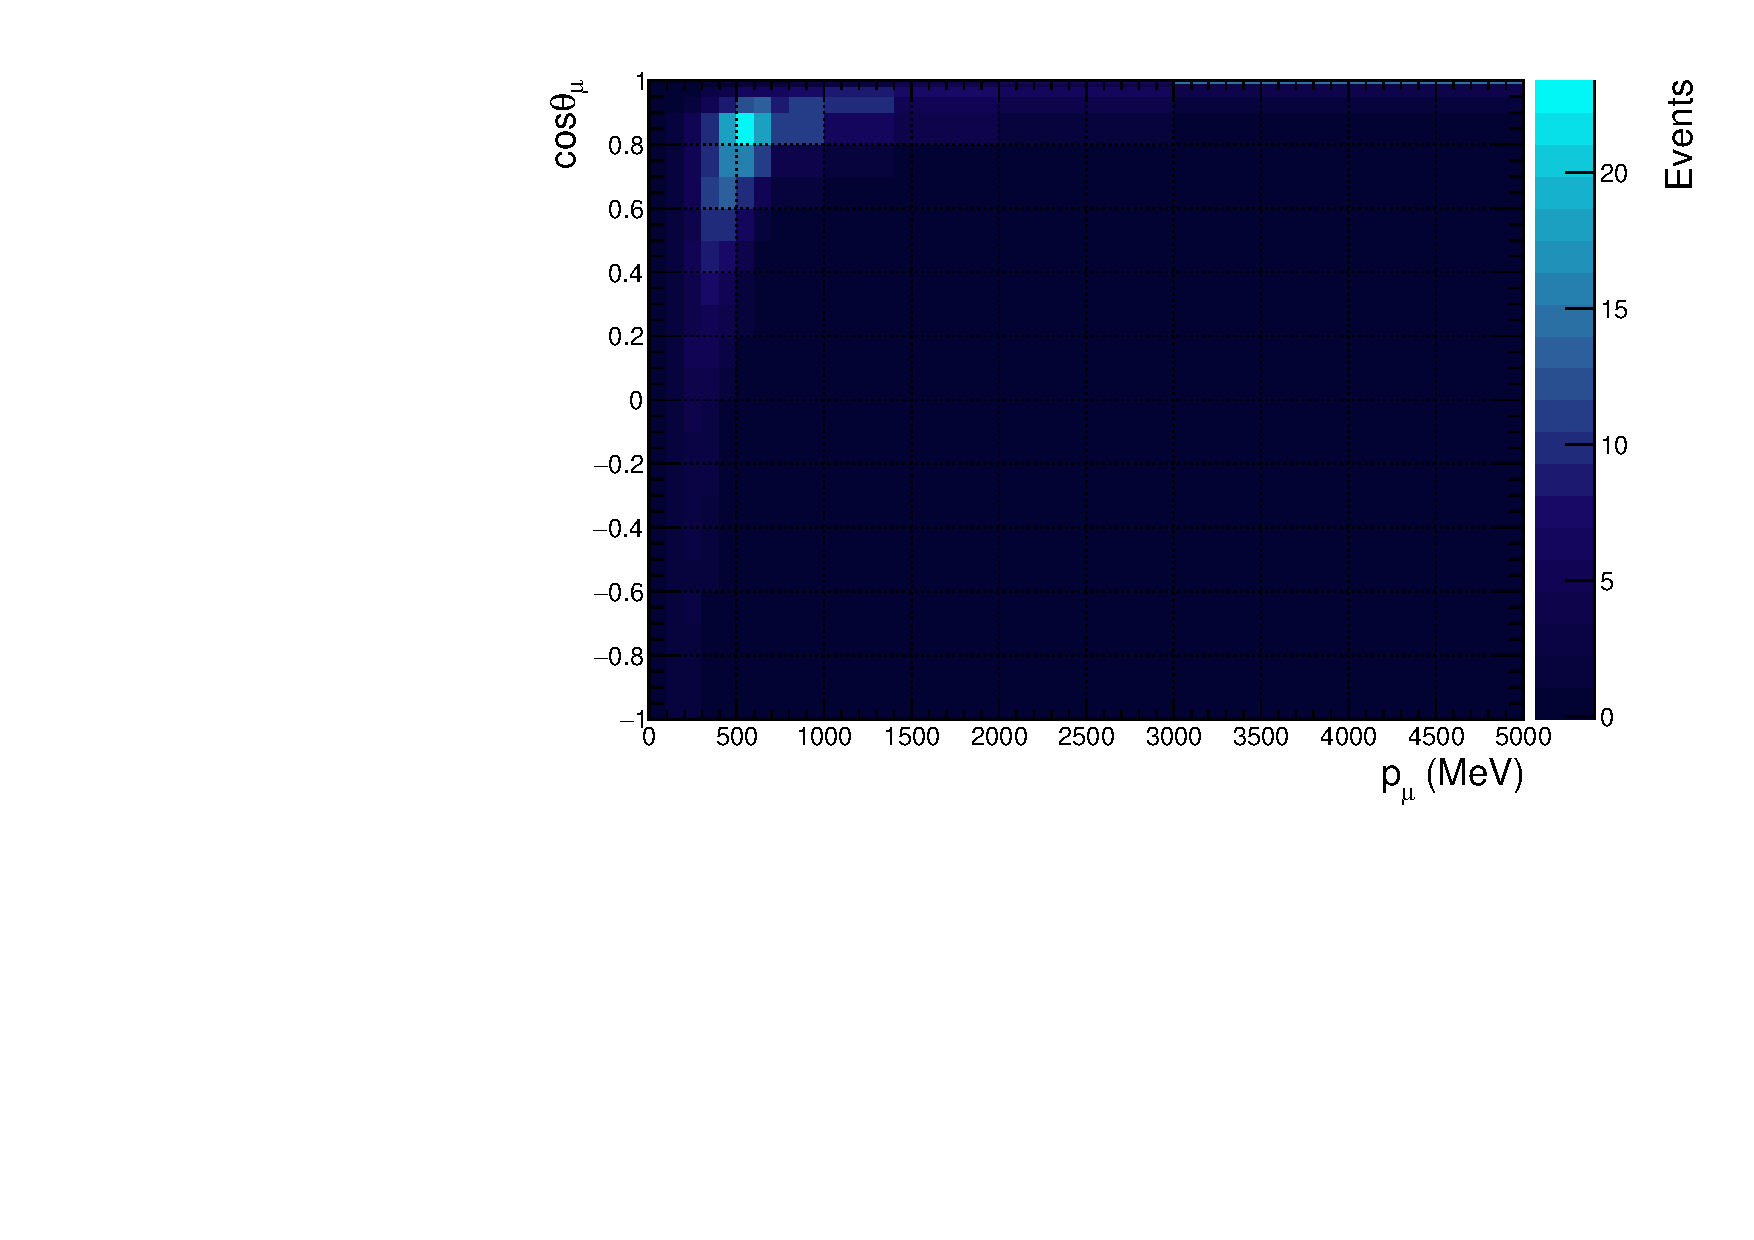
\includegraphics[width=0.9\linewidth]{figs/hptpc_sigvar_cc0pi0p.pdf}
  \caption{CC 0$\pi$ 0p: $p_{\mu}$-cos$\theta_{\mu}$}
\end{subfigure}
\begin{subfigure}{.49\textwidth}
  \centering
  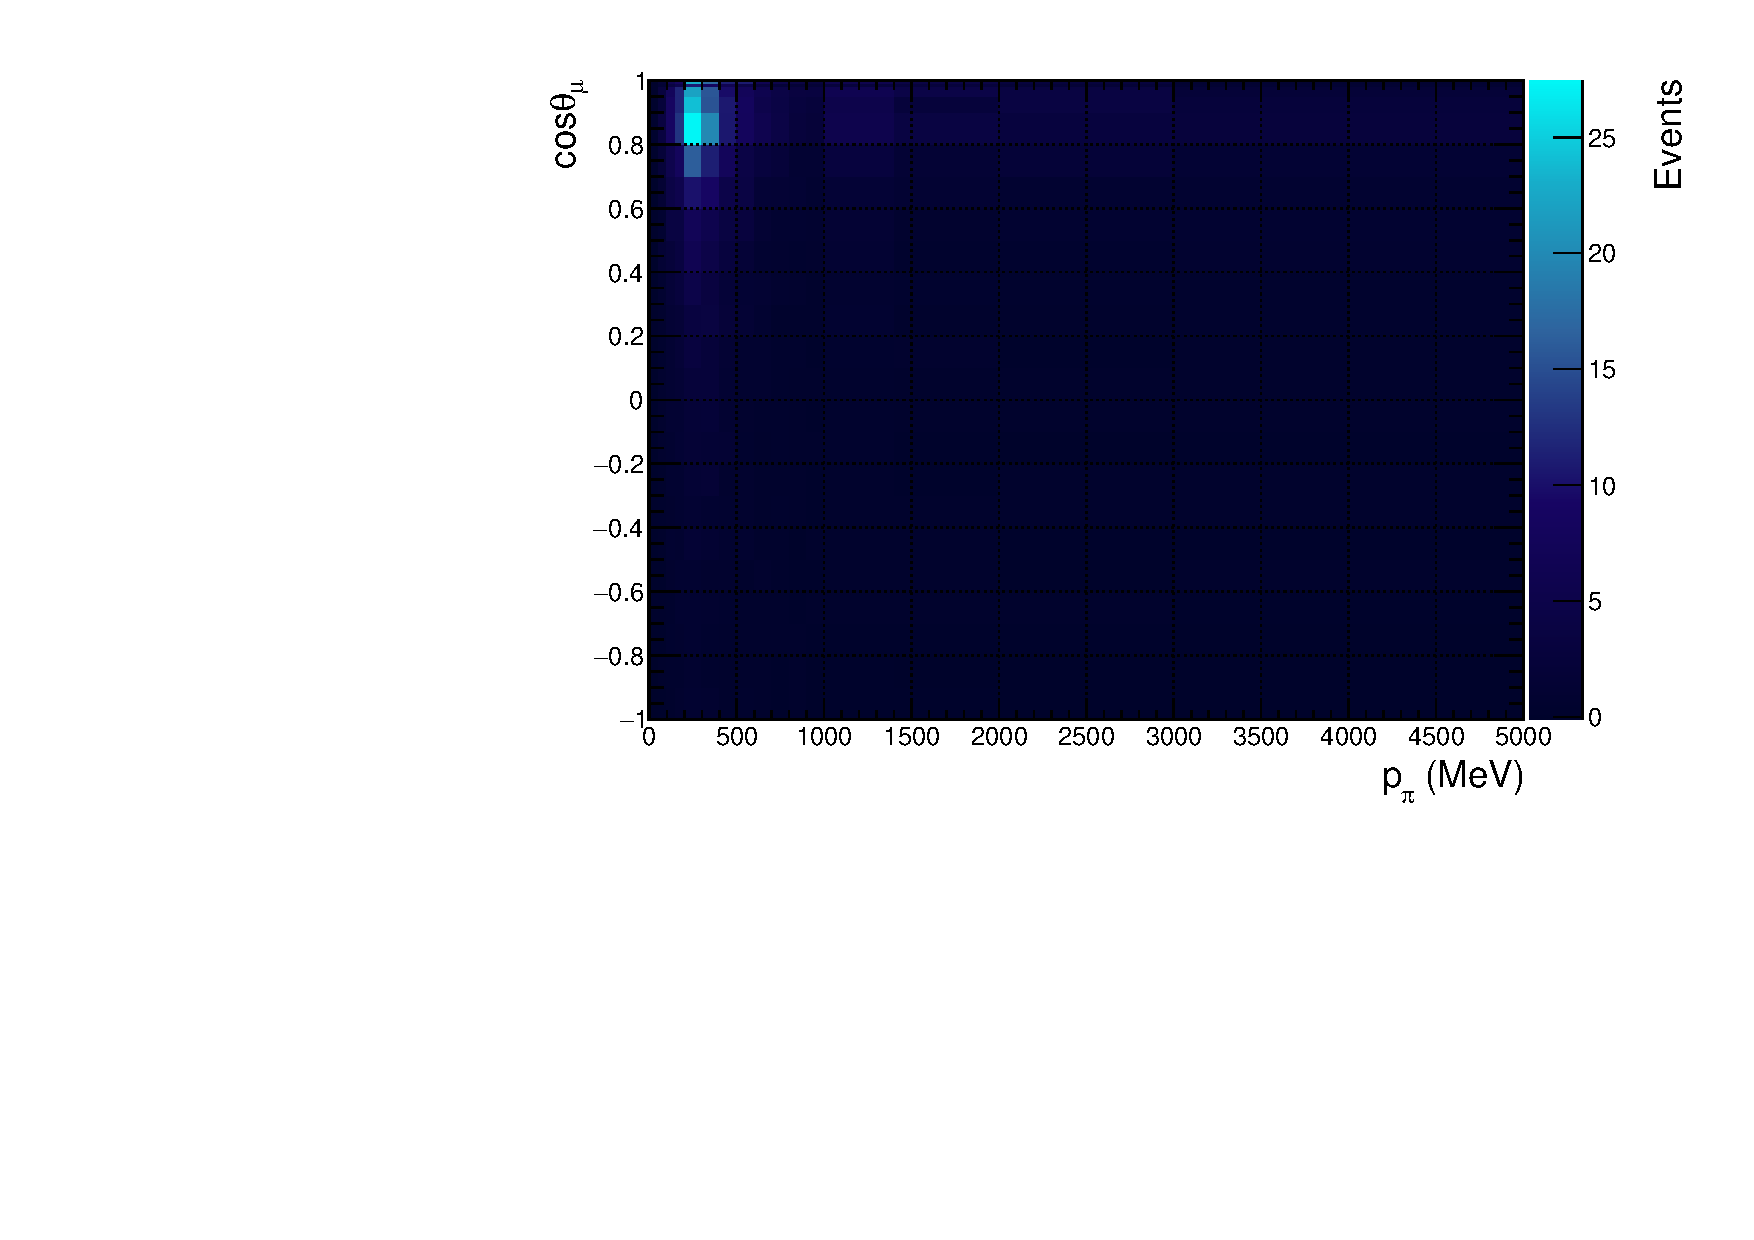
\includegraphics[width=0.9\linewidth]{figs/hptpc_sigvar_cc1pi0p.pdf}
  \caption{CC 1$\pi$ 0p: $p_{\pi}$-cos$\theta_{\mu}$}
\end{subfigure}
\begin{subfigure}{.49\textwidth}
  \centering
  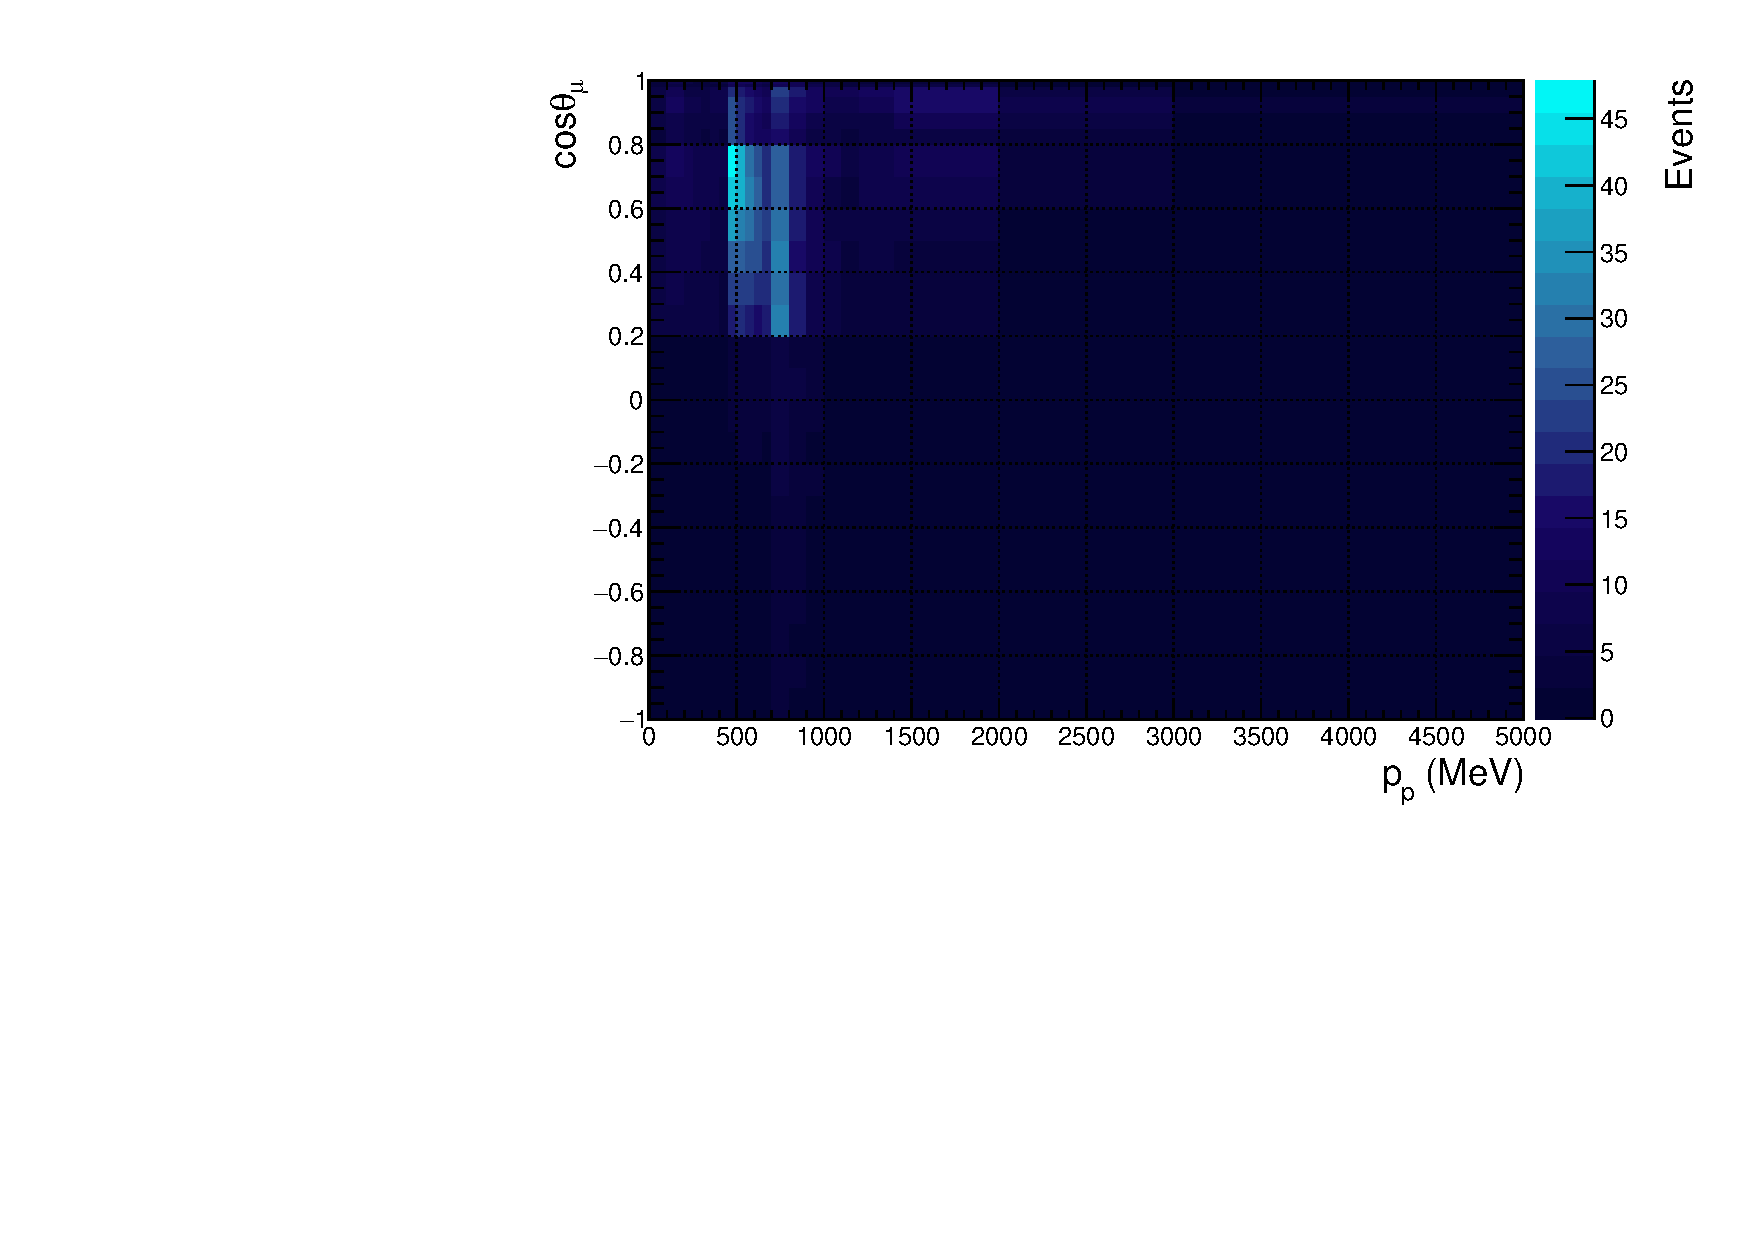
\includegraphics[width=0.9\linewidth]{figs/hptpc_sigvar_cc0pi1p.pdf}
  \caption{CC 0$\pi$ 1p: $p_{p}$-cos$\theta_{\mu}$}
\end{subfigure}
\begin{subfigure}{.49\textwidth}
  \centering
  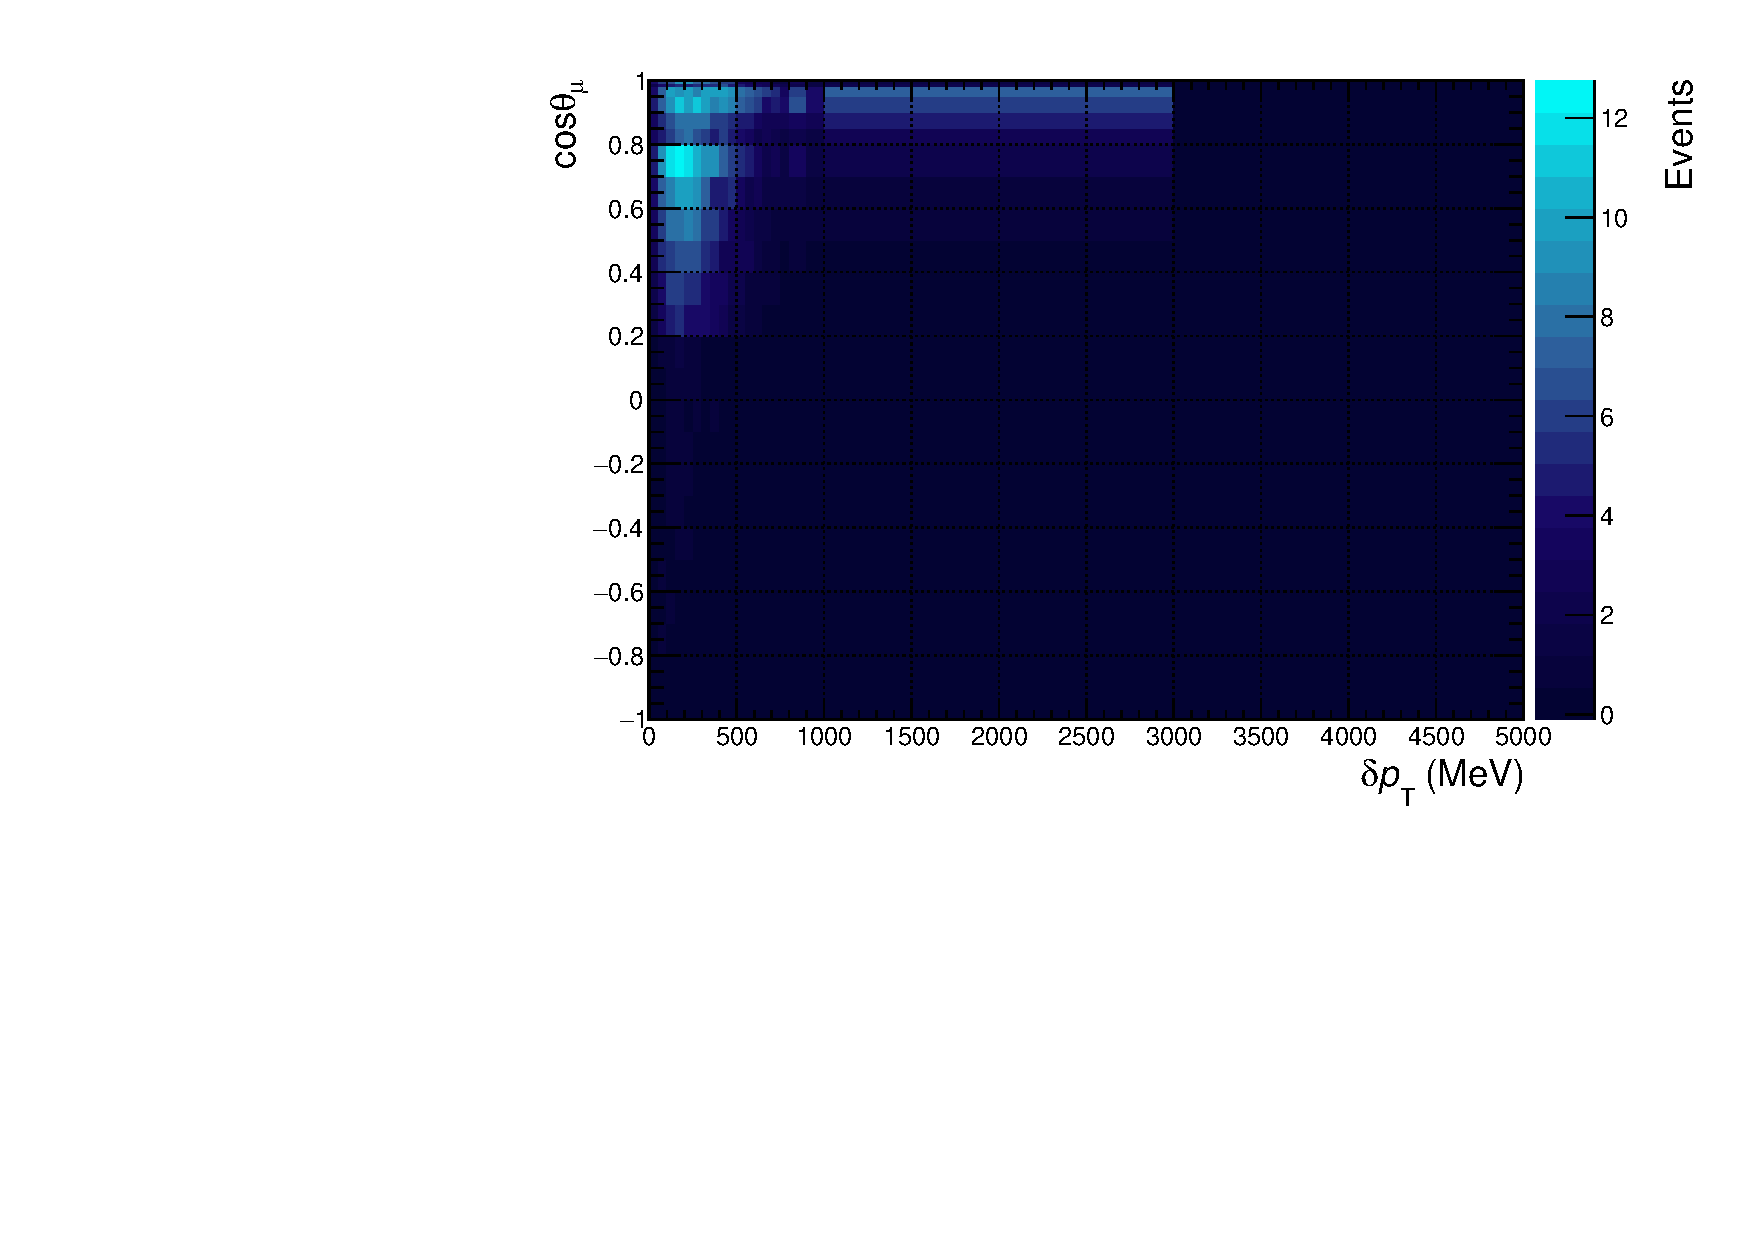
\includegraphics[width=0.9\linewidth]{figs/hptpc_sigvar_cc1pi1p.pdf}
  \caption{CC 1$\pi$ 1p: $\delta p_{T}$-cos$\theta_{\mu}$}
\end{subfigure}
\begin{subfigure}{.49\textwidth}
  \centering
  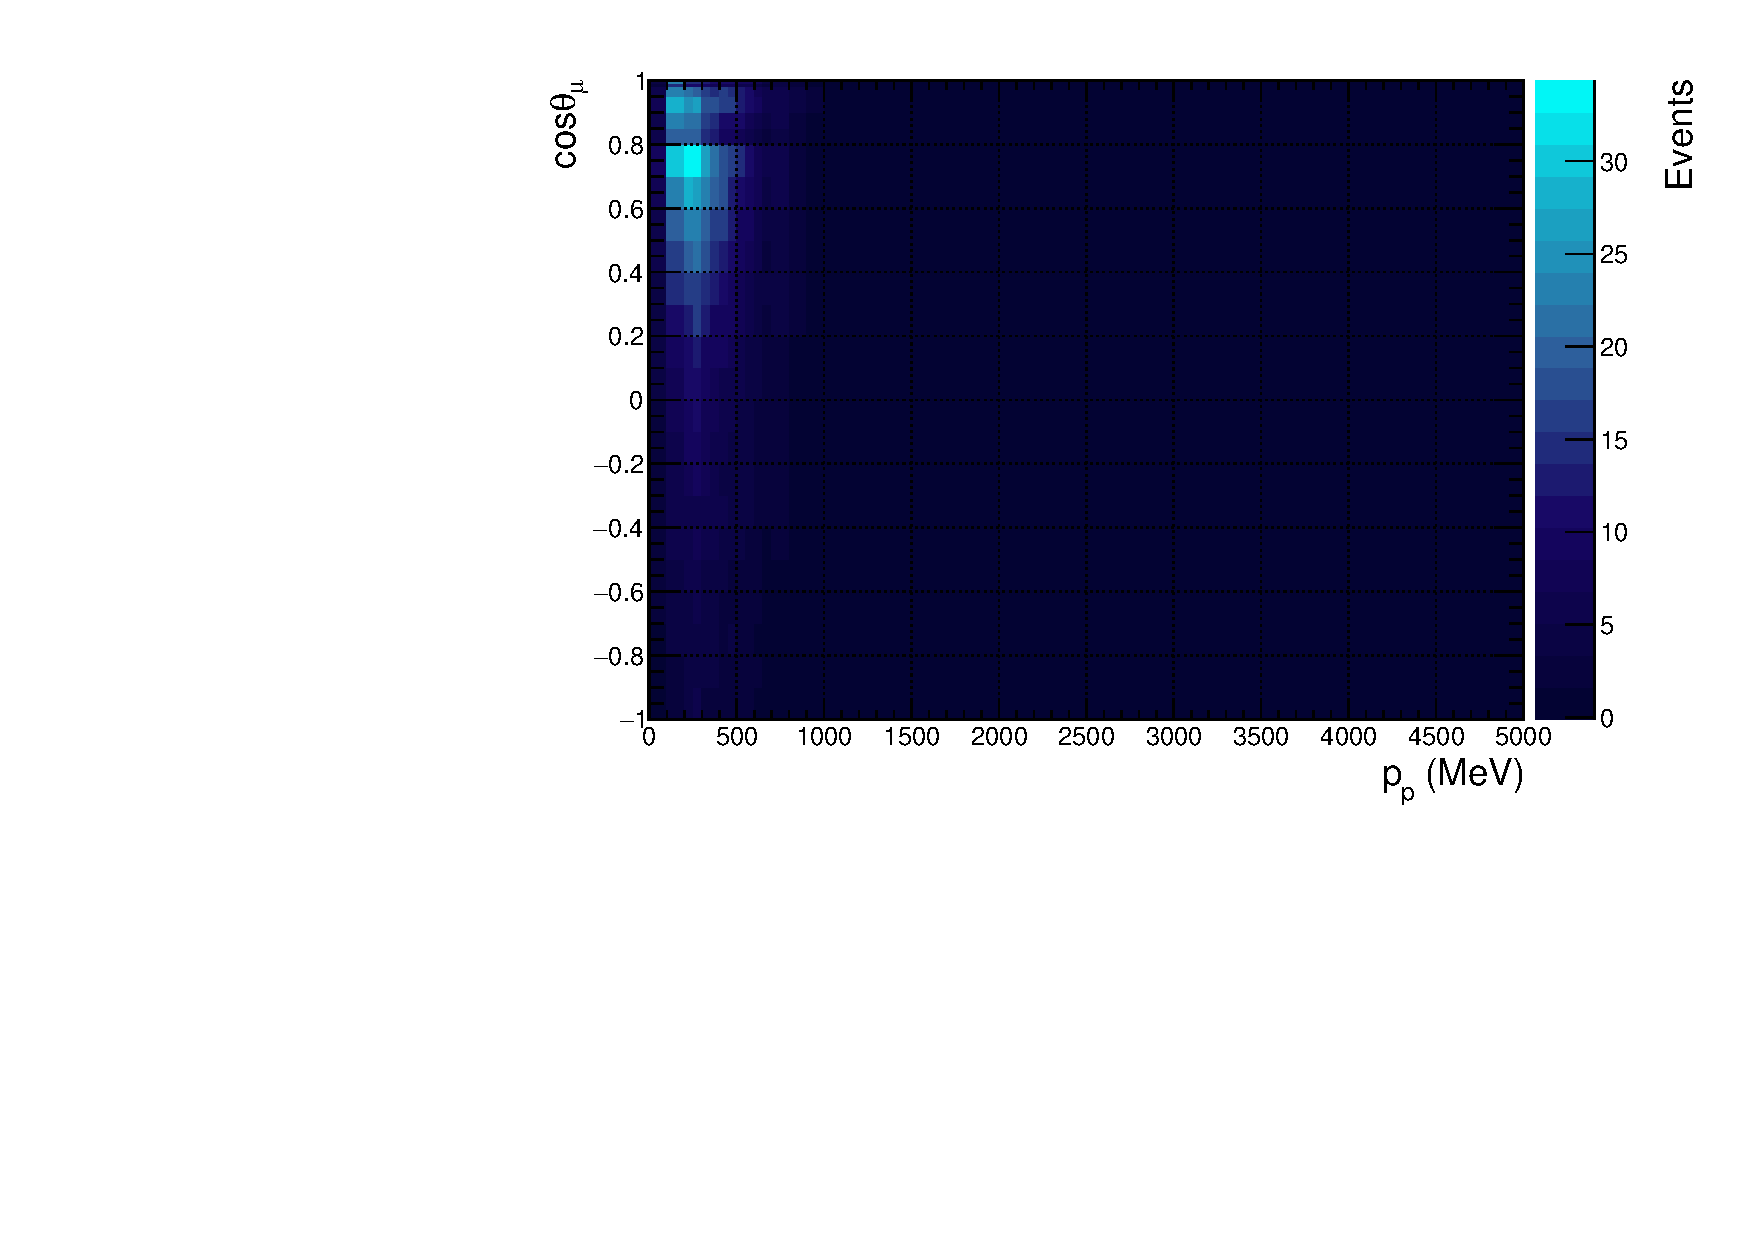
\includegraphics[width=0.9\linewidth]{figs/hptpc_sigvar_cc0piNp.pdf}
  \caption{CC 0$\pi$ Np: $p_{p}$-cos$\theta_{\mu}$}
\end{subfigure}
\begin{subfigure}{.49\textwidth}
  \centering
  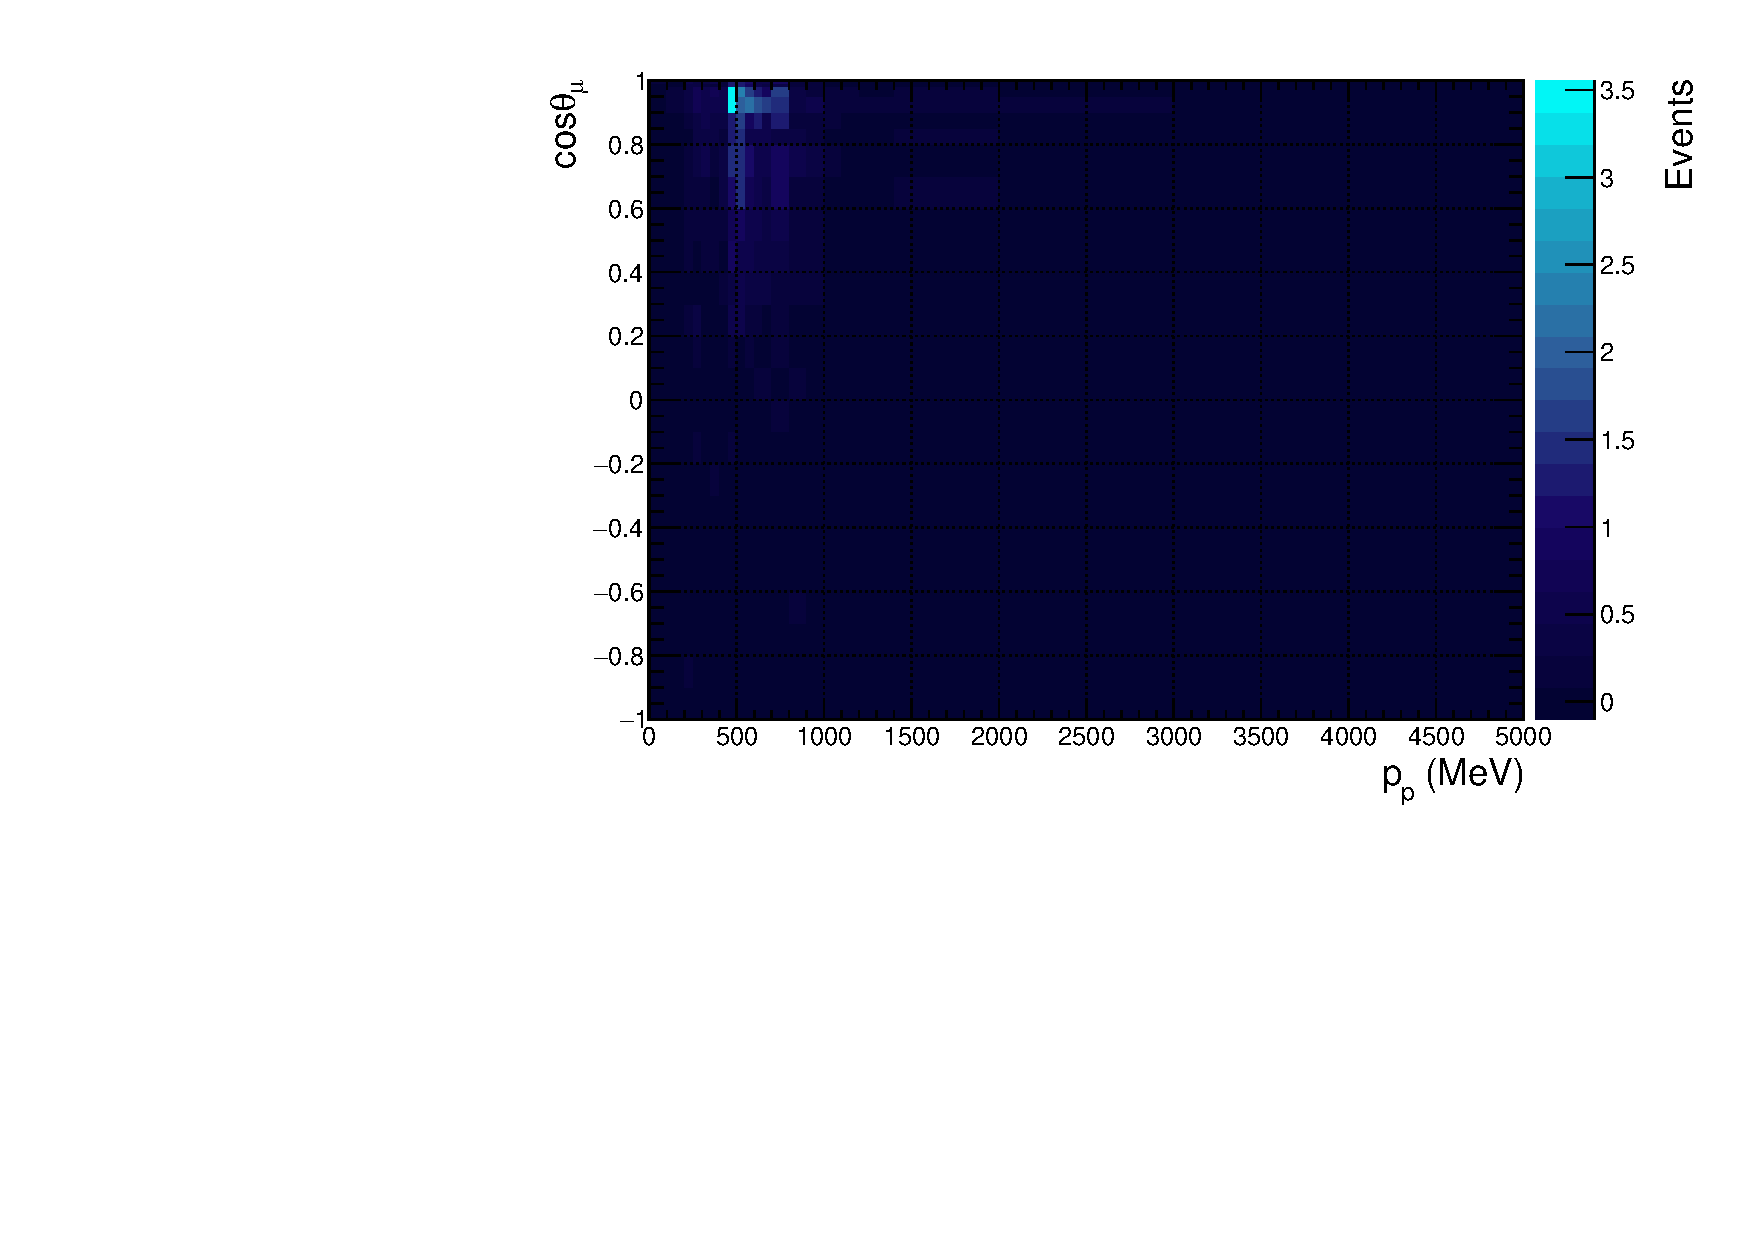
\includegraphics[width=0.9\linewidth]{figs/hptpc_sigvar_cc1piNp.pdf}
  \caption{CC 1$\pi$ Np: $p_{p}$-cos$\theta_{\mu}$}
\end{subfigure}
\begin{subfigure}{.49\textwidth}
  \centering
  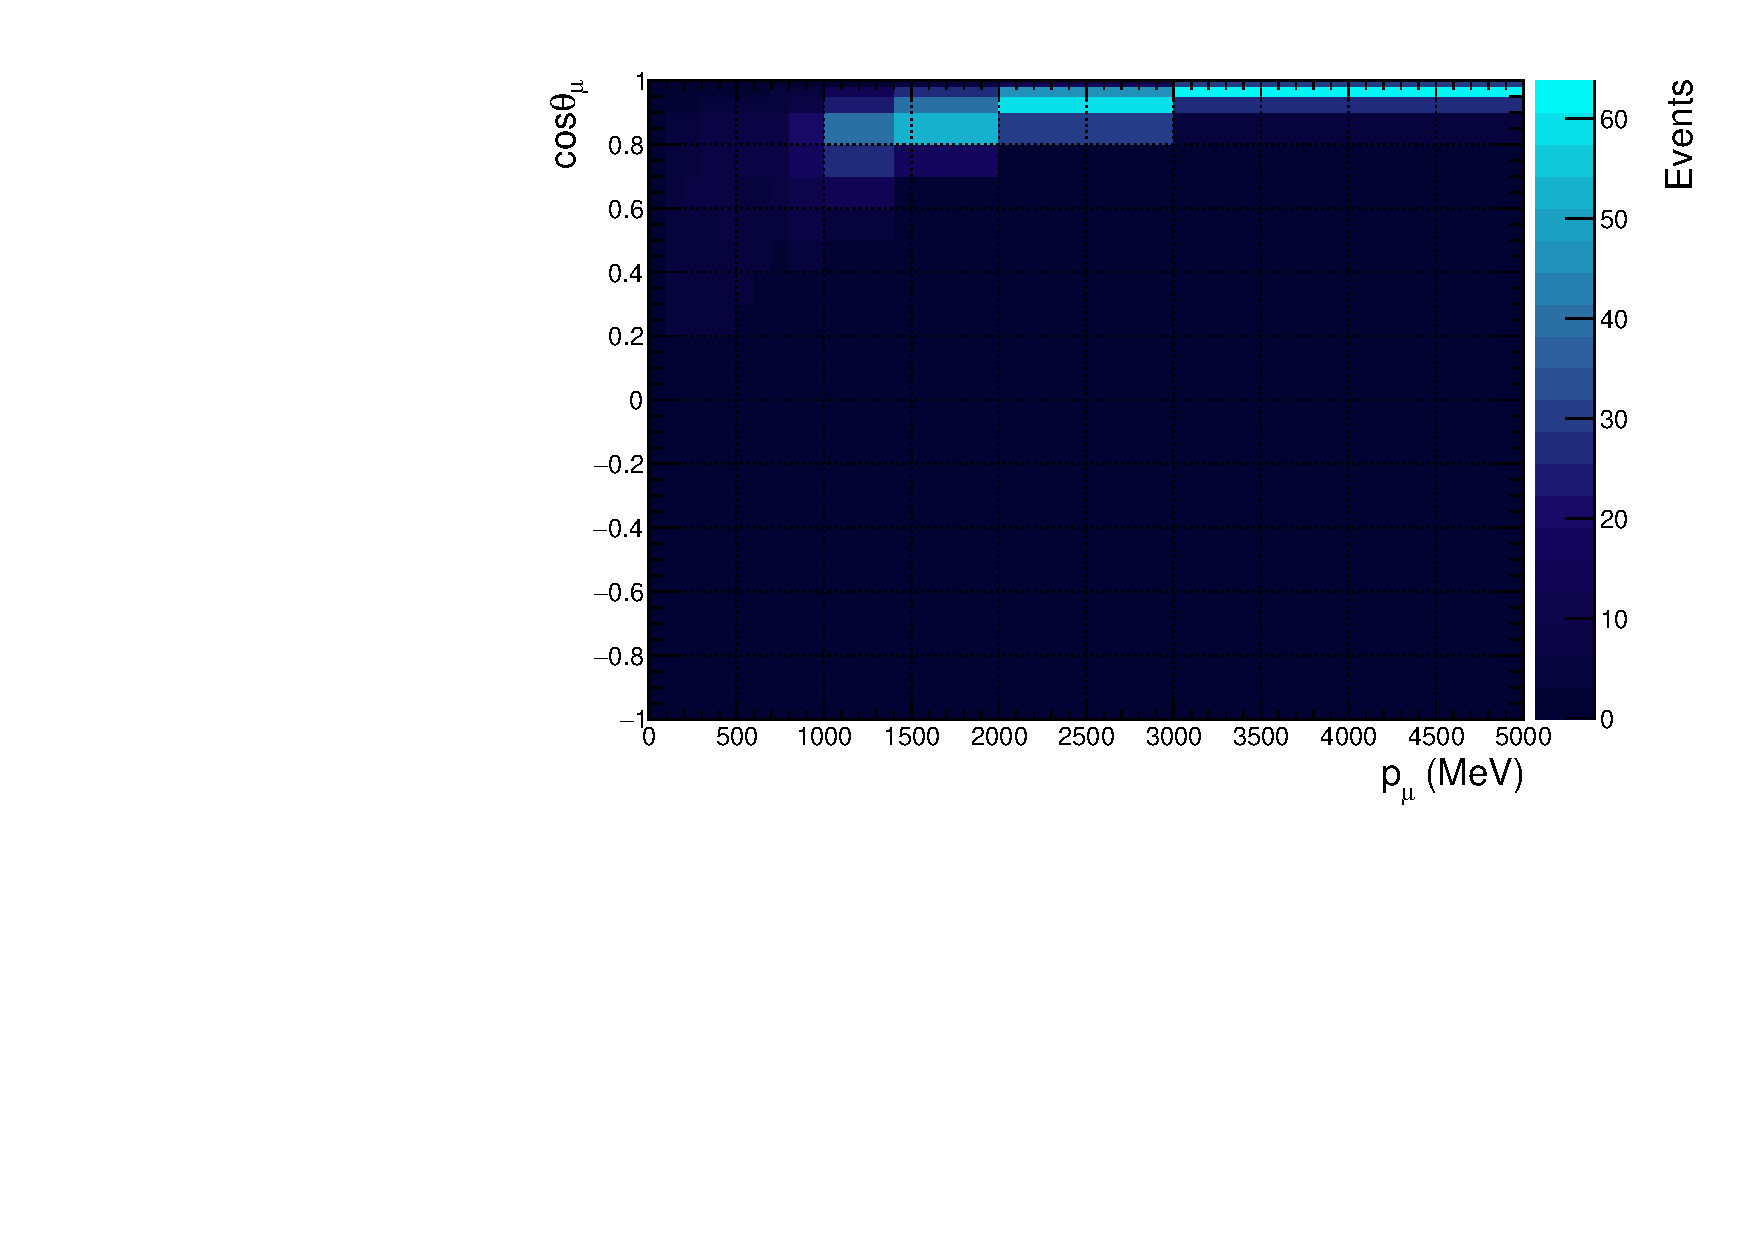
\includegraphics[width=0.9\linewidth]{figs/hptpc_sigvar_ccOther.pdf}
  \caption{CC Other: $p_{\mu}$-cos$\theta_{\mu}$}
\end{subfigure}
\caption{Distributions of HPTPC MC in different kinematic variables. For each sample, the pair of kinematics shown are those that had the largest change in event rates in $\pm1\sigma$ parameter variations.}
\label{fig:hptpcsigvar}
\end{figure}

The samples binned in $p_{p}$ and $p_{\pi}$ have hard cuts at low momentum, beyond which there are very few events. However, there are significantly below the ND280 detection thresholds. These samples, along with the $\delta p_{T}$ binned CC 1$\pi$ 1p  sample, have much narrower momentum distributions than those binned in $p_{\mu}$. The `gaps' in the distributions at cos$\theta_{\mu}\sim0.8$ are binning effects, whereby bins in the peak regions are finer, so have fewer events. The binnings have not been fully tuned to the new kinematic variables. 

\subsubsection{Asimov Fits}

Three Asimov fits were run to compare the sensitivities of the two detectors. The ND280 and HPTPC nominal MC distributions were fit in $p_{\mu}$-cos$\theta_{\mu}$, and the HPTPC MC was also fit mixture of different variables for each sample shown in Figure \ref{fig:hptpcsigvar}.

The fit results are shown in Figures \ref{} and \ref{}.

%Asimov in Pmu comp with STVs
%look at 1ds for 'problem' parameters?
%caveats: no det systs, low stats, events only on C, xs systs for lepton kin vars, hptpc will be bigger
%future studies: gas mixture, scale by size, 3 variables? 
\newpage